\documentclass[a4paper]{report}
\usepackage[utf8]{inputenc}
\usepackage[ngerman]{babel}
\usepackage{animate}
\usepackage{multicol}
\usepackage{amsmath, amsfonts, amsthm, graphicx, geometry, marvosym,esvect}%lipsum,
\geometry{verbose,a4paper,tmargin=25mm,bmargin = 25mm,lmargin=20mm }%,rmargin=20mm}
\usepackage{hyperref}
\usepackage{xcolor}

\usepackage{polynom}
\polyset{%
    vars=x,
    style=C,
    div=:,
    delims={(}{)}}
\usepackage{dsfont}
\colorlet{shadecolor}{yellow!15}
\usepackage{thmtools}
\hypersetup{colorlinks =true, linkcolor = blue, urlcolor =red, pdftitle={Mathematik in Q11}}
\usepackage{fancyvrb}
\usepackage{fancyhdr, lastpage}
\pagestyle{fancy}
\usepackage{xcolor}
\lhead{J. Gundelwein}
\rhead{Gymnasium Gröbenzell}
\cfoot{Seite \thepage \ von \pageref{LastPage}}
\usepackage[Sonny]{fncychap}
%Options: Sonny, Glenn, Lenny, Conny, Rejne, Bjarne, Bjornstrup
\usepackage{xcolor}
\definecolor{xvectorcolor}{HTML}{77933C}
\usepackage{afterpage}
\usepackage{tikz}
\usetikzlibrary{quotes, angles}
\usepackage[most]{tcolorbox}
\usepackage{pgfplots}
\pgfplotsset{compat=1.15, width =10cm}
\usepackage{mathrsfs}
\usetikzlibrary{arrows}
\newtcbtheorem[number within=section]{satz}
    {Satz}{colback=green!7,colframe=gray!85!black,fonttitle=\bfseries,title after break={Satz (Fortsetzung)}}{theorem}
\newtcbtheorem[number within=section]{defi}
    {Definition}{colback=red!7,colframe=red!45!black,fonttitle=\bfseries,title after break={Definition (Fortsetzung)}}{theorem}
\newtcbtheorem[number within=section]{bsp}
    {Beispiel}{colback=white,colframe=blue!70!green,fonttitle=\bfseries, breakable,title after break={Beispiel (Fortsetzung)}}{theorem}
    \newtcbtheorem[number within=section]{b8d}
    {Beachte}{colback=white,colframe=blue!60!green,fonttitle=\bfseries, breakable,title after break={Beachte (Fortsetzung)}}{theorem}
\newtcbtheorem[number within=section]{merke}{Merke} {colback=green!5,colframe=green!35!black,fonttitle=\bfseries, breakable,title after break={Merke (Fortsetzung)}}{theorem}
\newtcbtheorem[number within=section]{bem}
    {Bemerkung}{colback=red!2,colframe=red!35!black,breakable, fonttitle=\bfseries,title after break={Bemerkung (Fortsetzung)}}{theorem}
\usepackage{setspace}

\usepackage{multicol}
\usepackage{makeidx}
\renewcommand{\indexname}{Sachregister}
\makeindex
\usepgfplotslibrary{fillbetween}

% axis style, ticks, etc
\pgfplotsset{every axis/.append style={
              axis x line=middle,    % put the x axis in the middle
              axis y line=middle,    % put the y axis in the middle
              axis line style={<->}, % arrows on the axis
              xlabel={$x$},          % default put x on x-axis
              ylabel={$y$},          % default put y on y-axis
            %  axis equal,            % 1:1 ratio
              grid=both,             % coordinate grid
              grid style={line width=.1pt, draw=gray!10},
              major grid style={line width=.2pt,draw=gray!50},
              ticks=both,            % ticks for integers
              minor tick num=1,      % number of subticks
              ticklabel style={font=\small,fill=white},
              xlabel style={at={(ticklabel* cs:1)},anchor=north west},
              ylabel style={at={(ticklabel* cs:1)},anchor=south west},
            }
}
\tikzset{>=stealth}
\usepackage{eso-pic}
\newcommand\BackgroundPic{%
\put(0,0){%
\parbox[b][\paperheight]{\paperwidth}{%
\vfill
\centering
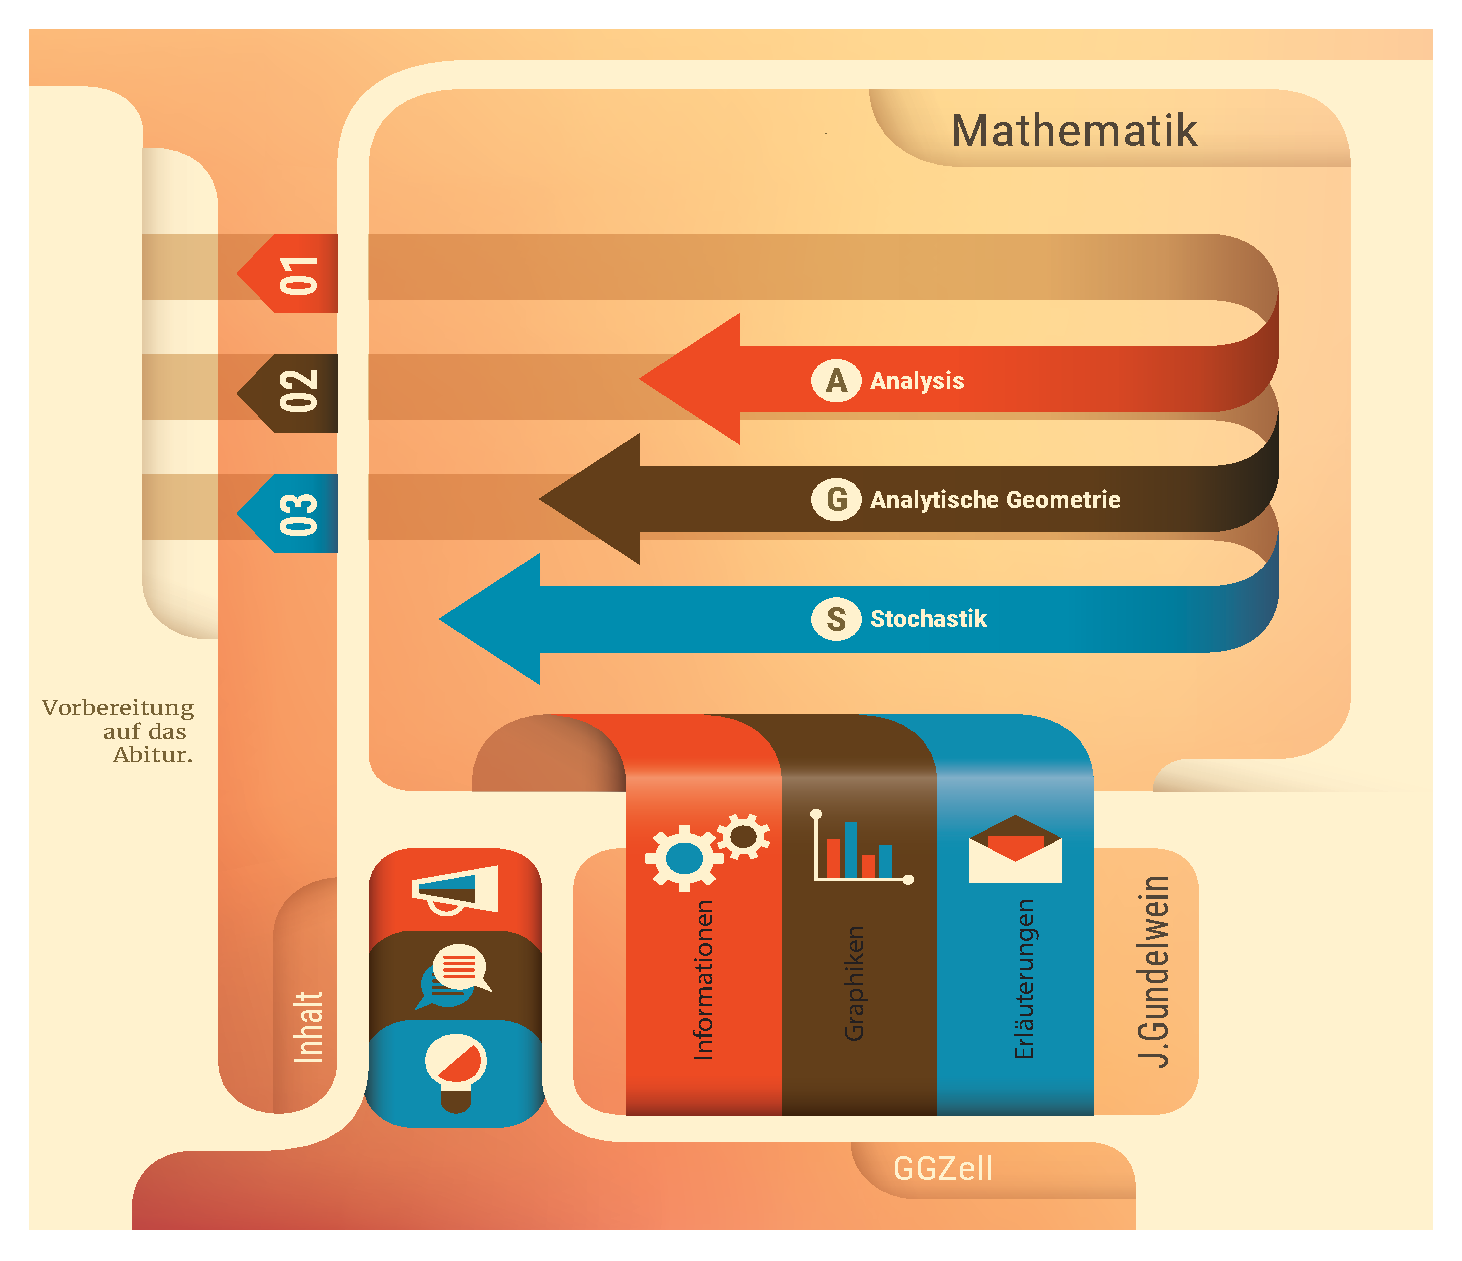
\includegraphics[width=\paperwidth,height=\paperheight,%
keepaspectratio]{Bilder/Anhang.pdf}%
\vfill
}}}
\begin{document}

\onehalfspacing
\begin{titlepage}

\begin{center}
%\renewcommand{\baselinestretch}{1}  % Zeilenabstand einfach
\huge \textbf{Gymnasium Gröbenzell}
\vspace{0.2cm}\\
\Large \textbf{ Mathematik Q11}
\vspace{1cm}\\
\LARGE \textbf{Abiturvorbereitung Mathematik}
\vspace{1cm}\\
\end{center}
\end{titlepage}
\tableofcontents
\newpage
\chapter{Analysis}
\begin{center}
\scalebox{2}{\begin{tikzpicture}
\begin{axis}[xmin= -2.2, xmax = 3.2, ymin= -3.2, ymax= 3.2,
        axis lines = middle, 
        ymajorgrids=true,
        xmajorgrids=true,
        xtick={-2, -1, 0, ..., 4},
        ytick={-4, -3, -2, ..., 3},
        xlabel = $x$,
        ylabel=$y$]
      \addplot[name path = f,red,thick,samples=200] {-1*(x-1)^2 +2};
      \addplot[name path = l1,teal,thick, samples = 200] {1/3*x^3-1.5};
      \addplot [
        thick,
        color=lightgray,
        fill=none, 
        fill opacity=0.5
      ]
      fill between[
        of=l1 and f,
        split,
        every segment no 2/.style={
            fill=lime,
        },
      ];
\end{axis}
\end{tikzpicture}}
\end{center}
\begin{section}{Lokales Differenzieren}\index{Differenzieren!lokal}
\begin{subsection}{Die mittlere Änderungsrate}
\begin{defi}{Die mittlere Änderungsrate}{maer}\index{Änderungsrate!mittlere}
Der Quotient $$\dfrac{\Delta y}{\Delta x} = \dfrac{f(b) - f(a)}{b - a}$$ heißt mittler Änderungsrate oder Differenzenquotient der Funktion f im Intervall $\left[a;b\right]$.\\
Geometrisch gedeutet ist der Differenzenquotient \index{Änderungsrate!Differenzenquotient} die Steigung der Sekante durch die Punkte $P(a|f(a))$ und $Q(b|f(b))$.
\end{defi}
\begin{bsp}{Ein Beispiel für die mittlere Änderungsrate}{bspmaer}
Gegeben sind die Punkte $P(3|4)$ und $Q(6|1)$ und damit die mittlere Änderungsrate: $$ \dfrac{\Delta y}{\Delta x} = \dfrac{4-1}{3-6} = \dfrac{3}{-3} = -1$$
\end{bsp}
\begin{bsp}{Graphische Darstellung der Sekantensteigung}{}
Gegeben ist die Funktion $f(x) =\dfrac{1}{2}x^3-x^2-2*x^1 +1$ mit $\mathds{D}_f =\mathds{R}$ und die Punkte $P(1|-1,51)$ und $Q(3,3|1,48)$. Um die mittlere Änderungsrate zu bestimmen muss jetzt die Steigung der Sekante berechnet werden.
$$m=\dfrac{\Delta y}{\Delta x} = \dfrac{y_2 -y_1}{x_2 -x_1} = \dfrac{1,48 -(-1,51)}{3,3 -1} = \dfrac{2,99}{2,3} = \dfrac{13}{10} = 1,3 $$
\begin{center}
\begin{tikzpicture}
\begin{axis}[xmin= -3.5, xmax = 4.5, ymin= -4, ymax= 4,
        axis lines = middle, 
        ymajorgrids=true,
        xmajorgrids=true,
        xtick={-3, -2, -1, 0, ..., 4},
        ytick={-4, -3, -2, ..., 3},
        xlabel = $x$,
        ylabel=$y$]
            \addplot[color= black, samples = 300, domain= -2:3.5]{0.5*x^3-x^2-2*x^1 +1};
           \draw[color = red] (1,-1.51)--(3.3,1.48);
           \draw[color = red] (3.3,-1.51)--(3.3,1.48);
           \draw[color = red] (1,-1.51)--(3.3,-1.51);
           \draw (1,-1.51)-- ++(-2.5pt,-2.5pt) -- ++(5pt,5pt) ++(-5pt,0pt) -- ++(5pt,-5pt) node[left] {P};
           \draw (3.3,1.48)-- ++(-2.5pt,-2.5pt) -- ++(5pt,5pt) ++(-5pt,0pt) -- ++(5pt,-5pt) node[right] {Q};
           \draw (3.3,-1.51)-- ++(-2.5pt,-2.5pt) -- ++(5pt,5pt) ++(-5pt,0pt) -- ++(5pt,-5pt);
            \draw[color = red] (2.2,0.5) node[left] {$\dfrac{\Delta y}{\Delta x} = 1,3$};
\end{axis}
\end{tikzpicture}
\end{center}
\end{bsp}
\end{subsection}
\subsection{Definition der Ableitung}
Die mittlere Änderungsrate beschreibt die durchschnittliche Steigung des Graphen einer Funktion zwischen zwei bestimmten Punkten. Die Ableitung realisiert den Übergang von der Sekante zur Tangente.
\begin{merke*}{Wichtige Informationen zur Definition  der Ableitung}
\index{Ableitung!Definition}
\begin{itemize}
 \item Nähern sich die Funktionswerte $f(x)$ einer Funktion $f$ einer Zahl $a$ beliebig genau an, das ist der Fall wenn sich die Werte für $x$ von links und von rechts an $x_0$ beliebig genau annnähern, so heißt $a$ Grenzwert der Funktion $f(x)$. Kurzschreibweise: $\lim_{x \rightarrow x_0} f(x)= a$ 
 \item Der Punkt Q laufe auf einer Kurve von links und rechts auf den Punkt P zu. Ergibt sich dabei ein gemeinsamer Grenzwert der Sekante, heißt die Grenzgerade Tangente an die Kurve im Punkt P.
 \item Die Steigung eines Graphen im Punkt P ist gleich der Steigung der Tangente in diesem Punkt.
\end{itemize}
\end{merke*}
Um die Ableitung zu definieren, betrachten wir die Normalparabel mit der Gleichung $$ y=x^2 $$ und darauf einen Punkt $P(1,5|2,25)$. Zur Bestimmung der Sekantensteigung bildet man den Differenzenquotienten zwischen dem Punkt $P$ und einem weiteren beliebigen Punkt $Q(x|x^2)$. 
\begin{bem*}{Differenzenquotient für $f(x) =x^2 $}\index{Änderungsrate!Differenzenquotient}
  
  $$ m_s(x)= \dfrac{\Delta y}{\Delta x} = \dfrac{f(x) - 2,25}{x - 1,5} = \dfrac{x^2 - 2,25}{x- 1,5} = \dfrac{(x-1,5)(x+1,5)}{x-1,5} =x+1,5 $$
Nähert sich der Punkt $Q$ beliebig nahe an den Punkt $P$ an, so unterscheidet sich die Steigung der Sekante immer weniger von 3. Man spricht in diesem Fall auch von einem Grenzwert.
$$\lim_{x\rightarrow 1,5} m_s(x) = 3$$
\end{bem*}

\label{hmethode}
\begin{merke*}{Die h-Methode zur Berechnung der Steigung }{}\index{Ableitung!h-Methode}
Wir führen eine Hilfsvariable h ein, diese gibt die Abweichung der Koordinate $x$ von der Koordinate $x_0$ angibt. Damit ist $x=x_0 + h$. Mit dieser Überlegung ist es jetzt möglich den Grenzwert zu bestimmen: $$m_t =\lim_{h\rightarrow 0} m_t(x_0 +h) =\lim_{h\rightarrow 0} \dfrac{f(x_0 + h) - f(x_0)}{h}.$$
\end{merke*}
\begin{defi}{}{} \index{Ableitung!Definition}
    Der Grenzwert des Differenzenquotienten $\dfrac{\Delta y}{\Delta x}$ für $x\rightarrow x_0$ heißt Differentialquotient oder Ableitung der Funktion $f$ an der Stelle $x_0$ und wird mit $f'(x_0)$ bezeichnet. Es gilt der Zusammenhang:$$f'(x_0) = \lim_{x\rightarrow x_0} \dfrac{f(x) - f(x_0)}{x - x_0} = \lim_{h\rightarrow 0} \dfrac{f(x_0 +h) - f(x_0)}{h}$$
\end{defi}
\begin{bem*}{}{}
Mit Hilfe der h-Methode ist es damit möglich jede beliebige Funktion abzuleiten. Man spricht in dem Fall von der Ableitung an einer bestimmten Stelle $x_0$. 
\end{bem*}
\begin{bsp}{Graphische Interpretation der h-Methode}{}
  \begin{center}
\begin{tikzpicture}
\begin{axis}[xmin= -0.2, xmax = 3.5, ymin= -1.5, ymax= 5.5,
        axis lines = middle, 
        ymajorgrids=true,
        xmajorgrids=true,
        xticklabels=\empty,
        yticklabels=\empty,
        xlabel = $x$,
        ylabel=$y$]  
        \addplot[color= black, samples = 300, domain= -2:2.5]{x^2};
        \draw[color= red] (1,-0.2) node[right] {$x_0$};
        \draw (1,0)-- ++(-2.5pt,-2.5pt) -- ++(5pt,5pt) ++(-5pt,0pt) -- ++(5pt,-5pt);
        \draw[color= red] (2,-0.2) node[right] {$x_0 +h$};
        \draw (2,0)-- ++(-2.5pt,-2.5pt) -- ++(5pt,5pt) ++(-5pt,0pt) -- ++(5pt,-5pt);
        \draw[color= red] (0,1.3) node[right] {$f(x_0)$};
        \draw (0,1)-- ++(-2.5pt,-2.5pt) -- ++(5pt,5pt) ++(-5pt,0pt) -- ++(5pt,-5pt);
        \draw[color= red] (0,4.3) node[right] {$f(x_0 + h)$};
        \draw (0,4)-- ++(-2.5pt,-2.5pt) -- ++(5pt,5pt) ++(-5pt,0pt) -- ++(5pt,-5pt);
         \draw[color= red] (2,4) node[right] {$Q$};
        \draw (2,4)-- ++(-2.5pt,-2.5pt) -- ++(5pt,5pt) ++(-5pt,0pt) -- ++(5pt,-5pt);
         \draw[color= red] (1,1) node[right] {$P$};
        \draw (1,1)-- ++(-2.5pt,-2.5pt) -- ++(5pt,5pt) ++(-5pt,0pt) -- ++(5pt,-5pt);
            \draw[red, dashed] (0,1 )-- (2,1);
            \draw[red, dashed] (2,0) -- (2,4);
            \draw[red, dashed] (0,4) -- (2,4);
            \draw[red, dashed] (1,0) -- (1,1);
         \draw[color= red] (1.5,0.7) node[right] {$h$};
         \addplot[color= red,dashed, samples = 300, domain= 0.5:2.5]{3*x - 2};
         \draw (1.4,-0.5) node[right] {$\Longleftarrow$};
         \draw[red] (1.3,-0.8) node[right] {$h\longrightarrow 0$};
\end{axis}
\end{tikzpicture}
\end{center}
 Das bedeutet, dass sich die beiden Punkten der Sekante beliebig genau annähern, ihr Abstand geht damit gegen Null ($h\rightarrow 0$). Somit wird aus der Sekannte eine Tangente.
\end{bsp}
\index{Änderungsrate!lokale}
\begin{bem*}{Tangentensteigung}{}
   Die Ableitung $f'(x_0)$ ist die Steigung der Tangente an den Graphen von $f$ an der Stelle $x_0$. Die Ableitung ist hierbei ein Maß dafür, wie stark sich die Funktionswerte in einer Umgebung um die Stelle $x_0$ ändern. Bei zeitlichen  Vorgängen spricht man von einer \textcolor{red}{momentanen Änderungsrate}, bei anderen Vorgängen von einer \textcolor{red}{lokalen Änderungsrate}.
\end{bem*}
\index{Änderungsrate!Steigungswinkel}
\index{Steigungswinkel}
\begin{bem*}{Der Steigungswinkel}{}
Der \textcolor{red}{Steigungswinkel} $\alpha$ einer Tangente ist der \textcolor{red}{spitze} Winkel zur x-Achse. Der Tangens des Steigungswinkels $\alpha$ ist gleich der Steigung $m$:$$\tan{(\alpha)} = m$$ \begin{center}
    bzw.
\end{center} $$\alpha = \arctan{(m)} = \tan^{-1}{(m)}$$
ist $m$ positiv, ist $\alpha$ positiv; ist $m$ negativ, ist $\alpha$ negativ. 
\begin{center}
\begin{tikzpicture}
\begin{axis}[xmin= -2, xmax = 3.5, ymin= -1.5, ymax= 3.5,
        axis lines = middle, 
        xticklabels=\empty,
        yticklabels=\empty,
        xlabel = $x$,
        ylabel=$y$]
        \addplot[red, samples = 100]{x^3+1};
        \addplot[blue, samples = 100]{3*x-1};
        \draw[color= red] (0.8,2.5) node[right] {$P$};
          \draw (1,2)-- ++(-2.5pt,-2.5pt) -- ++(5pt,5pt) ++(-5pt,0pt) -- ++(5pt,-5pt);

          \draw (1,0) coordinate (a) -- (0.33,0) coordinate (b) -- (1,2) coordinate (c)  pic[ draw = blue, fill = red!25!white, ->, angle eccentricity =1.2, angle radius = 1cm] {angle = a--b--c};
        \draw[color= black] (1,0.6) node[right] {$\alpha$};
\end{axis}
\end{tikzpicture}
\end{center}
\end{bem*}
Mit Hilfe dieser Definitionen und Überlegungen ist es nun möglich die Steigung einer Funktion an einer bestimmten Stelle zu berechnen und den dazugehörigen Steigungswinkel der Tangente zu bestimmen. Anhand eines Beispiels wird dieses jetzt exempkarisch durchgeführt.
\begin{bsp*}{Berechnung der Steigung und Steigungswinkel}{}
Gegeben ist die Funktion $f(x)= 2x^2 - 3x +2 $ und dem Definitionsbereich $\mathds{D}_f = \mathds{R}$. Wir betrachten die Stelle $x_0 = \dfrac{3}{2}$.
\begin{enumerate}
    \item Bestimmung der ersten Ableitung mit Hilfe der h-Methode
    \item Berechnung der Steigung an einer bestimmten Stell $x_0$
    \item Berechnung des Steigungswinkels der Tangente an dieser Stelle am Graphen
\end{enumerate}
\begin{equation*}
\begin{split}
f'(x_0) &= \lim_{h\rightarrow 0} \dfrac{f(x_0+h)-f(x_0)}{h}\\ f'(1,5)&=\lim_{h\rightarrow 0} \dfrac{f(1,5 +h) - f(1,5)}{h}\\ &= \lim_{h\rightarrow 0} \dfrac{2\cdot (1,5 +h)^2 -3\cdot(1,5+h) + 2-(2\cdot (1,5)^2 - 3\cdot (1,5) + 2)}{h}\\
&= \lim_{h\rightarrow 0} \dfrac{2\cdot (2,25 +3h + h^2) -3\cdot(1,5+h) + 2 - (4,5 -2,25 +2)}{h}\\
&= \lim_{h\rightarrow 0} \dfrac{4,5+6h+2h^2-2,25-3h+2-(4,5 -2,25 +2)}{h}\\
&= \lim_{h\rightarrow 0} \dfrac{2h^2+3h}{h}= \lim_{h\rightarrow 0} \dfrac{h\cdot( 2h+3)}{h} = \lim_{h\rightarrow 0} 2h+3\\
&= \textcolor{red}{3 = m_T} \hspace{0.3cm} \longrightarrow \hspace{0.3cm} \textbf{Steigung der Tangente}
\end{split}
\end{equation*}
Berechnung des Steigungswinkels der Tangente an der Stelle $x=1,5 $: 
\begin{equation*}
\begin{split}
\tan{(\alpha)} &= m\\
\tan{(\alpha)} &= 3\\
\alpha &= \arctan{(3)} \approx 71,57^{\circ}  
\end{split}
\end{equation*}
\end{bsp*}
\subsection{Differenzierbarkeit und Lineare Transformation}\index{Differenzieren!Differenzierbarkeit} \index{Ableitung!Differenzierbarkeit}
\begin{defi}{Die Differenzierbarkeit einer Funktion}{}
 Eine Funktion f heißt an der Stelle $x_0$ im Inneren des Definitionsbereichs $D_f$ differenzierbar, wenn der Grenzwert \begin{equation*}
     f'(x_0) =\lim_{h\rightarrow 0}\dfrac{f(x_0 +h) -f(x_0)}{h}
 \end{equation*} existiert, sich also bei links- und rechtsseitiger Annäherung der gleiche Wert ergibt. Der Grenzwert des Differenzenquotient heißt Differentialquotient.
\end{defi}
\begin{bsp*}{Die Überprüfung der Differenzierbarkeit mit der h-Methode}\index{Differenzieren!Differenzierbarkeit!Beispiel}
    Gegeben ist die Funktion $f(x)= x^2 + |x|$, wir überprüfen die Ableitung an der Stelle $P(0|f(0))$.

$$f(x)= \begin{cases}
              x^2 + x & \text{für}\hspace{0.5cm} x\geq 0\\
              x^2 - x & \text{für}\hspace{0.5cm}  x< 0 
         \end{cases}$$
Für die Untersuchung der Differenzierbarkeit sind folgende Grenzwerte zu überprüfen::
\begin{equation*}
\begin{split}
f'(0) &= \lim_{h\rightarrow0^-} \dfrac{f(0+h)-f(0)}{h}\\ &=\lim_{h\rightarrow 0^-} \dfrac{(0+h)^2 - (0+h) -0}{h}\\ &= \lim_{h\rightarrow 0^-} \dfrac{h^2-h}{h} = \lim_{h\rightarrow 0^-} h-1=-1 
\end{split}
\end{equation*}
\begin{equation*}
\begin{split}
f'(0)&=\lim_{h\rightarrow 0^+}\dfrac{f(0+h)-f(0)}{h}\\
&=\lim_{h\rightarrow 0^+} \dfrac{(0+h)^2 + (0+h) -0}{h}\\ 
&=\lim_{h\rightarrow 0^+} \dfrac{h^2 + h}{h} = \lim_{h\rightarrow 0^+} h+1 =1
\end{split}
\end{equation*}
Der Differenzenquotient hat daher für $x\rightarrow 0$ keinen Grenzwert, die Funktion $f$ ist damit an der Stelle $x_0 = 0$ nicht differenzierbar. Der Graph $G_f$ hat an dieser Stelle einen "`Knick"'.
\end{bsp*}

\begin{bem*}{}\index{Differenzieren!Differenzierbarkeit!Lineare Transformationen}\index{Lineare Transformation}
Die Lineare Transformation der Betragsfunktion ändert nichts an der Nicht-Differenzierbarkeit der Funktion.
\end{bem*}
Während der letzten Schuljahre wurden verschiedene Funktionsarten einer linearen Transformation unterzogen. Als Beispiel wird hier auf die Funktionen: 
 \begin{equation*}
    \begin{split}
        f(x) &= x^2\\
        g(x) &= \sin{(x)}\\
        h(x) &= \cos{(x)}
    \end{split}
\end{equation*}
verwiesen.\\ 
In Jahrgangsstufe 9 wurde die Normalparabel auf unterschiedlichste Arten transformiert. In der 10. Jahrgangsstufe wurden Trigonometrischen Funktionen transformiert.
\begin{bsp*}{Transformationen am Bespiel der Normalparabel}{}\index{Lineare Transformation!Beispiel}
Der Graph der Funktion $f(x) = x^2$ läßt sich wie folgt transformieren:
\begin{itemize}
\item $g_1(x) = -x^2$ $\Longrightarrow$ Normalparabel an der $x-$Achse gespiegelt
\item $g_2(x) =   x^2 +a$ $\Longrightarrow$ $G_f$  Richtung der y--Achse um a verschoben
\item $g_3(x) =(x-a)^2$ $\Longrightarrow$ $G_f$ in Richtung der x--Achse um a verschoben
\item $g_4(x) =a\cdot x^2$ und $a>0$, $\Longrightarrow$ $G_f$ in Richtung der y--Achse mit dem Faktor a gestreckt bzw. gestaucht
\end{itemize}
\end{bsp*}

\begin{merke}{Allgemeine Darstellung der Linearen Transformationen} 
Die lineare Transformation lässt sich allgemein wie folgt schreiben:\index{Lineare Transformation!allgemein}\\
Wir erhalten aus dem Graphen $G_f$ der Funktion f den Graphen der Funktion g mit:
\begin{itemize}
\item $g(x) = - f(x)$, indem man $G_f$ an der x--Achse spiegelt
\item $g(x) =f(-x)$, indem man $G_f$ an der y--Achse spiegelt
\item $g(x) = f(x) +a$ indem man $G_f$ in Richtung der y--Achse um a verschiebt
\item $g(x) =f(x-a)$ indem man $G_f$ in Richtung der x--Achse um a verschiebt
\item $g(x) =a\cdot f(x)$ und $a>0$, indem man $G_f$ in Richtung der y--Achse mit dem Faktor a streckt bzw. staucht
\item $g(x) =f(a\cdot x)$ und  $a>0$, indem man $G_f$ in Richtung der x--Achse mit dem Faktor $\dfrac{1}{a}$ staucht bzw. streckt.

\end{itemize}
\end{merke}
\label{lintrans}
\end{section}

\begin{section}{Globales Differenzieren}\index{Differenzieren!global}
\subsection{Die Ableitungsfunktion}
\begin{defi}{Die Ableitungsfunktion}{ablf}
    \index{Ableitung!Ableitungsfunktion}
    Zu einer Funktion $f$ heißt die Funktion $f': x \mapsto f'(x)$ die Ableitungsfunktion oder kurz die Ableitung von $f$. Die Ableitung einer Funktion $f$ ist diejenige Funktion, die jeder Stelle $x$, an der $f$ differenzierbar ist, die Ableitung $f'(x)$ zuordnet:
$$f'(x)=\lim_{h\rightarrow 0} \dfrac{f(x + h) - f(x)}{h}.$$ 
\end{defi}
\begin{bem}{Bedeutung der Ableitungsfunktion}{bedeutungAblf}
   Die Ableitungsfunktion $f'$ beschreibt die Steigung der Funktion $f$ an jeder Stelle $x\in \mathds{R}$. \\
   Bei der Ableitung von Polynomen verringert sich der Grad der Funktion bei jeder Ableitung um 1.\\
\end{bem}
\begin{bsp}{Beispielfunktion}{}\index{Ableitung!Ableitungsfunktion!Beispiel}
Die Funktion $f(x) = x^3 + x^2 -2x+1$ mit $x\in\mathds{R}$ ist ein Polynom vom Grad 3, die Funktion $f'(x) = 3x^2+2x-2$ ist die erste Ableitung der Funktion $f(x)$. Die Graphen der beiden Funktionen ist unten gegeben. 
\definecolor{ccqqqq}{rgb}{0.8,0,0}
\begin{center}
\begin{tikzpicture}[line cap=round,line join=round,>=triangle 45,x=1cm,y=1cm]
\begin{axis}[
x=1cm,y=1cm,
axis lines=middle,
ymajorgrids=true,
xmajorgrids=true,
xmin=-4.6725325047810795,
xmax=3.4865844816315783,
ymin=-3.970650919871985,
ymax=4.84273488148887,
xtick={-4,-3,...,3},
ytick={-3,-2,...,4},]
\clip(-4.6725325047810795,-3.970650919871985) rectangle (3.4865844816315783,4.84273488148887);
\draw[line width=1.2pt,smooth,samples=100,domain=-4.6725325047810795:3.4865844816315783] plot(\x,{(\x)^(3)+(\x)^(2)-2*(\x)+1});
\draw[line width=1.2pt,color=ccqqqq,smooth,samples=100,domain=-4.6725325047810795:3.4865844816315783] plot(\x,{3*(\x)^(2)+2*(\x)-2});
\begin{scriptsize}
\draw[color=black] (-2,-2.7) node {$f(x)$};
\draw[color=ccqqqq] (-2.2,3.5) node {$f'(x)$};
\end{scriptsize}
\end{axis}
\end{tikzpicture}
\end{center}
\end{bsp}
\subsection{Ableitung ganzrationaler Funktionen}
Die Ableitung von Funktionen mit der h-Methode ist für jede Funktion möglich. Allerdings wird das Ableiten damit schnell mühsam. Durch die Anwendung von Regeln zur Ableitung ganzrationaler Funktionen wird das Bilden der ersten Ableitung um einiges einfacher.\\
\begin{merke*}{Ableitungsregel Potenzfunktionen}{}\index{Ableitung!Regel!Potenzfunktion}
Die Potenzfunktion $f$ mit $f(x) = x^n$ und natürlichen Exponenten $n$ ist differenzierbar und es gilt: $$f'(x) = n\cdot x^{n-1}$$
\underline{Merkregel:} Der Term $x^n$ wird differenziert, indem man den Exponenten $n$ als Faktor voranstellt und den Exponenten um 1 verringert.
\end{merke*}
\begin{bsp}{Beispiele für das Ableiten von Potenzfunktionen}{}
\begin{itemize}
    \item $f(x)= x^3\ \longrightarrow f'(x) = 3x^2$
    \item $g(x) = \dfrac{3}{4} x^5 \ \longrightarrow g'(x)=  5\cdot \dfrac{3}{4} x^4 = \dfrac{15}{4}x^4$ 
    \item $h(x) = x^{\pi} \ \longrightarrow h'(x) = \pi \cdot x^{\pi -1}$
\end{itemize}
\end{bsp} 
\begin{defi}{Die Normale}{}\index{Normale}
    Die Gerade, die im Berührpunkt auf der Tangente senkrecht steht, heißt Normale. Hierbei hängen die Steigung der Normalen und die Steigung der Tangente wie folgt zusammen $$m_{Normale} = -\dfrac{1}{m_{Tangente}}$$
\end{defi}

\subsection{Anwendung der Ableitungsfunktion-Newton-Verfahren}\index{Newton-Verfahren}

Innerhalb der Analysis ist die Bestimmung der Nullstellen eine der zentralen Aufgaben. Diese Berechnung erfolgt allerdings nur bei einer begrenzten Anzahl von Funktionsklassen problemlos. So gibt es bei Polynomen vom Grad $n\geq 4$ keine Lösungsformel\footnote{Für den Grad $n=2$ ist die Lösungsformel die bereits bekannte Mitternachtsformel: $x_{1,2} = \dfrac{-b\pm \sqrt{b^2 -4ac}}{2\cdot a}$} mehr. Für den Grad $n\geq 4$ gibt es bei Polynomen dann verschiedene Wege die Nullstellen zu bestimmen. Eine dieser Möglichkeiten ist die Polynomdivision\footnote{Die Polynomdivision ist nicht Teil des Lehrplans der Klasse 11, allerdings aus der 10. Klasse bekannt.}, siehe hierzu auch \ref{polynomdivision}. Eine weitere Möglichkeit die Nullstellen zu bestimmen liefert das Newton-Verfahren. Hierbei ist es möglich, die Nullstellen beliebig genau näherungsweise zu bestimmen. \\
Funktionsweise des Newton-Verfahren:
\begin{merke*}{Iterationsverfahren}\index{Iterationsverfahren}
  Für die Durchführung des Newton-Verfahrens werden bestimmte Rechenschritte beliebig oft wiederholt. Da sich dabei die Rechenschritte nur mit sich ändernden Zahlen wiederholen, handelt es sich um ein iteratives Verfahren.
\end{merke*}
Um das Newton-Verfahren zu verstehen, betrachtet man die allgemeine Herleitung. Ziel des Verfahren ist es, eine Nullstelle einer beliebigen Funktion $f$ zu finden. Setzt man einen Anfangswert $x_0$ in die Funktionsgleichung ein, erhält man im Allgemeinen einen von Null verschiedenen Funktionswert $f(x_0)$. Bildet man jetzt die Tangente durch den Punkt $A(x_0|f(x_0))$ am Graphen $G_f$ der Funktion $f$ und bestimmt davon die Nullstelle erhält man im Allgemeinen eine bessere Näherung für die Nullstelle des Graphen $G_f$\footnote{Ein Besipiel für das Bestimmen einer Tangentengleichung findet man im Beispiel \ref{Tangentengleichung}}. 
\begin{bsp*}{Herleitung des Newton-Verfahren}\index{Newton-Verfahren!Herleitung}
    Gegeben ist eine beliebige Funktion $f$ und ein Startwert $x_0 \in \mathds{D}_f$ und $A(x_0|f(x_0))$ mit $f'(x_0)\neq 0$. Für die Tangente durch $x_0$ an $G_f$ gilt allgemein folgende Geradengleichung $y_T= m\cdot x + t$. Am Punkt $A(x_0|f(x_0))$ ergibt sich damit folgende Gleichung:$$y_T = f'(x_0) \cdot x + t.$$ Um die Nullstelle dieser bestimmten Tangente bestimmen zu können, ist es notwendig, dass man den y-Achsenabschnitt bestimmt. Hierfür werden die Werte $x_0$ und $f(x_0)$ in die Geradengleichung eingesetzt und nach $t$ aufgelöst. 
    \begin{equation*}
	\left.\begin{aligned}
	f(x_0) &= f'(x_0) \cdot x_0 + t \\
	t &= f(x_0) - f'(x_0) \cdot x_0 
	\end{aligned}
	\right\}
\quad \text{Tangentengleichung:}\hspace{0.1cm } y_T = f'(x_0) \cdot x + (f(x_0) - f'(x_0) \cdot x_0 )
\end{equation*}
Um die erste Näherung zu bekommen, wird die Nullstelle der Tangentengleichung berechnet.
    \begin{equation*}
	\left.\begin{aligned}
	0 &=  f'(x_0) \cdot x + (f(x_0) - f'(x_0) \cdot x_0 ) \\
	f'(x_0) \cdot x &= f'(x_0)\cdot x_0  - f(x_0)\\
    x &=\dfrac{f'(x_0)\cdot x_0  - f(x_0)}{f'(x_0)}
	\end{aligned}
	\right\}
\quad \text{Näherungswert:}\hspace{0.1cm } x = x_0 -\dfrac{f(x_0)}{f'(x_0)}
\end{equation*}
\end{bsp*}
\begin{defi}{Das Newton-Verfahren}{}\index{Newton-Verfahren!Definition}
    Ist $x_n$ ein Näherungswert einer Nullstelle der Funktion $f$ und $f'(x_n)\neq 0$, dann ist $$x_{n+1} = x_n -\dfrac{f(x_n)}{f'(x_n)}$$ im Allgemeinen ein besserer Näherungswert.
\end{defi}
\begin{bem}{Konvergenz des Newton-Verfahren}{}\index{Newton-Verfahren!Konvergenz}
    Das Newton-Verfahren konvergiert nicht immer. Die Konvergenz der Iteration hängt vom Startwert $x_0$ ab. Hierbei bedeutet der Begriff Konvergenz, dass sich die Näherungswerte der eigentlichen Nullstelle immer genauer annähern.
\end{bem}
\begin{bsp}{Die Funktion $f(x)= x^3 -2x^2-x+1$}{}
Am Beispiel der Funktion $f(x)=x^3-2x^2-x+1$ soll das Newton-Verfahren exemplarisch durchgeführt werden. Als Startwert wird die Stelle $x_0 = 1,24$ gewählt. Um die Iteration durchführen zu können, muss die erste Ableitung $f'$  der Funktion $f$ gebildet werden, diese lautet $f'(x)= 3x^2 -4x -1$. Nun ist es möglich, die einzelnen Iterationschritte durchzuführen.
\begin{center}$\begin{aligned}
	x_n &= x_{n-1}-\dfrac{f(x_{n-1})}{f'(x_{n-1})} \\
	x_0 &= 1,24\\
    x_1 &= x_0 - \dfrac{f(x_0)}{f'(x_0)}\\
    &=1,24 - \dfrac{f(1,24)}{f'(1,24)}\\
    &=1,24 - \dfrac{-1,41}{-1,3472}\\
    &=\dfrac{4093}{21050}\approx 0,19\\
    x_2&= 0,64
	\end{aligned}$\end{center}
\begin{center}
    \begin{tikzpicture}
        \begin{axis}[xmin= -3.5, xmax = 4.5, ymin= -4, ymax= 4,
        axis lines = middle, 
        ymajorgrids=true,
        xmajorgrids=true,
        xtick={-3, -2, -1, 0, ..., 4},
        ytick={-4, -3, -2, ..., 3},
        xlabel = $x$,
        ylabel=$y$]
            \addplot[color= black, samples = 300, domain= -2:3]{x^3-2*x^2-x^1 +1};
            \addplot[color= black, samples = 300, domain= -1:3]{-1.35*x^1 +0.27};
            \draw[dashed] (1.24,-1.41)  -- (1.24,0) node(xline)[above] {$x_0$};
            \draw (1,-1.5)   node[left] {$A$};
            \draw (1.2390888331407657,-1.4073470487766349)-- ++(-2.5pt,-2.5pt) -- ++(5pt,5pt) ++(-5pt,0pt) -- ++(5pt,-5pt);
            \draw[dashed] (0.2,0.2) node(xline)[above] {};
            \draw (0.1,-0.6)   node [above] {$x_1$};
            \draw[dashed] (0.2,0)  -- (0.2,0.73) node(xline)[right] {$f(x_1)$};
            \draw (0.2,0.73)-- ++(-2.5pt,-2.5pt) -- ++(5pt,5pt) ++(-5pt,0pt) -- ++(5pt,-5pt);
        \end{axis}
    \end{tikzpicture}     
\end{center}
\end{bsp}
Die einzelnen Iterationsschritte sind hierbei nicht immer von einzeln durchzuführen. Mit den aktuell erlaubten Taschenrechnern ist es möglich, die sich wiederholenden Schritte immer wieder durchzuführen\footnote{Siehe Anleitung Taschenrechner für die Programmierung.}.
\end{section}
\section{Kurvendiskussion}
 \subsection{Monotonie und Extrema}   
 \begin{defi}{Monotonie}{}\index{Kurvendiskussion!Monotonie}\index{Monotonie}
 Es sei $f$ eine Funktion auf einem Intervall $I$ definiert. Gilt für alle $x_1, x_2 \in I$ mit $x_1<x_1:$
 \begin{equation*}
	\left.\begin{aligned}
	f(x_1) &<  f(x_2)  \\
	f(x_1) &> f(x_2)
	\end{aligned}
	\right\}
\quad \text{So nennt man f}
	\quad\left\{\begin{aligned}
	\text{monoton steigend}  \\
	\text{monoton fallend}
	\end{aligned}
\right\}
\quad
 \text{im Intervall I} 
\end{equation*} 
 \end{defi}
 \begin{defi}{Extrema}{}
   Es sei $f$ eine auf einem Intervall $I$ definierte Funktion. Dann nennt man $f(x_0)$ \textcolor{red}{lokales Maximum} wenn es eine Umgebung $U$ um $x_0$ gibt, sodass für alle  $x \in U \in \mathds{D_f}$ gilt: \textcolor{red}{$f(x_0)\geq f(x)$}. Der Punkt \textcolor{red}{$P(x_0|f(x_0))$} heißt dann \textcolor{red}{Hochpunkt (HoP)}.\\
   Es sei $f$ eine auf einem Intervall $I$ definierte Funktion. Dann nennt man $f(x_0)$ \textcolor{red}{lokales Minimum} wenn es eine Umgebung $U$ um $x_0$ gibt, sodass für alle  $x \in U \in \mathds{D_f}$ gilt: \textcolor{red}{$f(x_0)\leq f(x)$}. Der Punkt \textcolor{red}{$P(x_0|f(x_0))$} heißt dann \textcolor{red}{Tiefpunkt (TiP)}.
 \end{defi}
 \begin{satz}{Bedingung für die Monotonie}{}\index{Monotonie!Bedingung}
 Ist die Funktion $f$ im Intervall $I$ eine differenzierbare Funktion und 
  \begin{equation*}
	\left.\begin{aligned}
	f'(x) &>0  \\
	f'(x) &<0
	\end{aligned}
	\right\}
\quad \text{für alle $x\in I$, dann ist $f$ in $I$ streng monoton}
	\quad\left\{\begin{aligned}
	\text{wachsend}  \\
	\text{fallend}
	\end{aligned}
\right.
\end{equation*} 
 \end{satz}
 \begin{satz}{Notwendige Bedingung für innere Extrempunkt}{}\index{Monotonie!Notwendige Bedingung}
   Eine Funktion $f$ und ihre Ableitung $f'$ seien auf einem Intervall $I$ definiert. Dann gilt: \textcolor{red}{Hat} $f$ an einer inneren Stelle $x_0\in I$ einen \textcolor{red}{Extremwert}, so ist \textcolor{red}{$f'(x_0)=0$}
 \end{satz}
 \begin{b8d}{Vorzeichenwechsel und Extrema}{}\index{Monotonie!Vorzeichenwechsel}
 Die Art der einzelnen Extrema läßt sich leicht durch die Vorzeichenwechsel (VZW) der Ableitung bestimmen.
 \begin{itemize}
\item Hochpunkt (HoP) $HoP(x_0|f(x_0))$ genau dann, wenn es einen VZW der Ableitung von \textcolor{red}{positiv nach negativ} gibt
\begin{enumerate}
    \item $f'(x_0) = 0$
    \item $x_i<x_0 \Rightarrow f'(x_i)>0$
    \item $x_0 <x_i \Rightarrow f'(x_i)<0$
\end{enumerate}
\item Tiefpunkt (TiP) $TiP(x_0|f(x_0))$ genau dann, wenn es einen VZW der Ableitung von \textcolor{red}{negativ nach positiv} gibt
\begin{enumerate}
    \item $f'(x_0) = 0$
    \item $x_i<x_0 \Rightarrow f'(x_i)<0$
    \item $x_0 <x_i \Rightarrow f'(x_i)>0$
\end{enumerate}
\item Terrassenpunkt (TP) $TP(x_0|f(x_0))$
\begin{enumerate}
    \item $f'(x_0) = 0$
    \item \textcolor{red}{kein VZW}
\end{enumerate}
 \end{itemize}
 \end{b8d}
 \begin{bsp}{Bestimmung der Monotonie und der Extrema I}{}
 Gegeben ist die Funktion $f(x) = 2x^3 +6x^2 -2x + 1$ mit $\mathds{D}_f = \mathds{R}$ und der ersten Ableitung $f'(x) = 6x^2+12x-2$.\\
 Vorgehen:
 \begin{enumerate}
     \item Bestimmung der Nullstelle der ersten Ableitung
     \item Untersuchung der Monotonie mit Hilfe der Monotonietabelle
     \item Entscheidungen zu möglichen Extrema
 \end{enumerate}
 \begin{center}$\begin{aligned}
	f'(x)&= 6x^2+12x-2\\
    0 &= 6x^2+12x-2\\
    x_{1,2} &= \dfrac{-12 \pm \sqrt{144 +48} }{12} = \dfrac{-12\pm 8\sqrt{3}}{12}\\
    &= \dfrac{-3\pm 2\sqrt{3}}{3}\\
    x_1&= \dfrac{-3+ 2\sqrt{3}}{3}\\
    x_2&= \dfrac{-3 - 2\sqrt{3}}{3}
	\end{aligned}$\end{center}
 Mit diesen beiden Nullstellen ist es möglich eine faktorisierte Form des Funktionsterms aufzuschreiben. $$f'(x)= 6x^2+12x-2 = 6\cdot \left(x-x_1 \right)\cdot \left(x-x_2 \right)$$
Monotonietabelle:\\
\begin{center}\begin{tabular}{||c|c|c|c|c|c||}
    \hline
    $x$& $ -\infty <x<x_2 $ & $ x_2 \approx -2.15$ &$ x_2<x<x_1 $ & $x_1 \approx 0,15 $& $ x_1<x<\infty $\\
    \hline \hline
    $6\cdot (x-x_2)$ & - &  0 & - &  & +  \\
    \hline
    $(x -x_1)$ & - & & + &0 & + \\
    \hline
    $f'(x)$ & + & 0 & - & 0 & +\\ 
    \hline
    $G_f$ & smw & HoP & smf & TiP & smw\\
    \hline
\end{tabular}
\end{center}
\begin{center}
    \begin{tikzpicture}
        \begin{axis}[xmin= -4.1, xmax = 2.5, ymin= -15.1, ymax= 20.5,
        axis lines = middle, 
        ymajorgrids=true,
        xmajorgrids=true,
        xtick={-4, -3.5, -3,  ..., 2},
        ytick={-15, -10, -5, ..., 20},
        xlabel = $x$,
        ylabel=$y$]
            \addplot[color= red, samples = 300, domain= -3.7:1.7]{2*x^3+ 6*x^2 -2*x+1};
         \draw (1.5,15)   node [right] {\textcolor{red}{$f(x)$}};  
            \addplot[color= black, samples = 300, domain= -3.7:1.7]{6*x^2+ 12*x -2};
            \draw (-3.5,12)   node [right] {$f'(x)$}; 
            \draw (-2.1,0)   node [above] {$x_2$};
            \draw (0.15,0.5)   node [left] {$x_1$};
             \draw (-2.15,0)-- ++(-2.5pt,-2.5pt) -- ++(5pt,5pt) ++(-5pt,0pt) -- ++(5pt,-5pt);
             \draw (-2.1,14)   node [above] {HoP};
              \draw (-2.15,13.15)-- ++(-2.5pt,-2.5pt) -- ++(5pt,5pt) ++(-5pt,0pt) -- ++(5pt,-5pt);
               \draw (0.15,0.84)-- ++(-2.5pt,-2.5pt) -- ++(5pt,5pt) ++(-5pt,0pt) -- ++(5pt,-5pt);
               \draw (0.15,4.5)   node [above] {TiP};
              \draw (0.15,0)-- ++(-2.5pt,-2.5pt) -- ++(5pt,5pt) ++(-5pt,0pt) -- ++(5pt,-5pt);
        \end{axis}
    \end{tikzpicture}  
\end{center}
\end{bsp}
\begin{bsp}{Bestimmung der Monotonie und der Extrema II}{}
Betrachtet wird die Funktion $f(x)= x^3-6x^2 +9x-2$ mit $\mathds{D}_f =\mathds{R}$ und der ersten Ableitung $f'(x)= 3x^2 -12x +9$
\begin{center}$\begin{aligned}
	f'(x)&= 3x^2 -12x +9\\
    0 &= 3x^2 -12x +9\\
    x_{1,2} &= \dfrac{12 \pm \sqrt{144 -8} }{6} = \dfrac{12\pm \sqrt{36}}{6} = \dfrac{12 \pm 6}{6} = 2\pm 1\\
    x_1&= 3\\
    x_2&= 1
	\end{aligned}$\end{center}
 Mit diesen beiden Nullstellen ist es möglich eine faktorisierte Form des Funktionsterms aufzuschreiben. $$f'(x)= 3x^2-12x+9 = 3\cdot \left(x-3 \right)\cdot \left(x-1 \right)$$

Monotonietabelle:\\
\begin{center}\begin{tabular}{||c|c|c|c|c|c||}
    \hline
    $x$& $ -\infty <x<1 $ & $ x_2 =1$ &$ 1<x<3 $ & $x_1 = 3 $& $ 3<x<\infty $\\
    \hline \hline
    $3\cdot (x-1)$ & - &  0 & - &  & +  \\
    \hline
    $(x -3)$ & - & & + & 0 & + \\
    \hline
    $f'(x)$ & + & 0 & - & 0 & +\\ 
    \hline
    $G_f$ & smw & $HoP(1|2)$ & smf & $TiP(3|-2) $& smw\\
    \hline
\end{tabular}
\end{center}
\begin{center}
    \begin{tikzpicture}
        \begin{axis}[xmin= -1.1, xmax = 5.5, ymin= -4.1, ymax=3.5,
        axis lines = middle, 
        ymajorgrids=true,
        xmajorgrids=true,
        xtick={-4, -3, -2,  ..., 5},
        ytick={-4, -3, -2, ..., 3},
        xlabel = $x$,
        ylabel=$y$]
            \addplot[color= red, samples = 300, domain= -0.2:4.2]{x^3-6*x^2+9*x-2};
     \addplot[color= black, samples = 300, domain= -0.2:4.2]{3*x^2-12*x+9};
            \draw (4.2,2)   node [right] {$f(x)$}; 
            \draw (1,3)   node [right] {$f'(x)$}; 
            \draw (1.2,0)   node [above] {$x_2$};
            \draw (2.8,0)   node [above] {$x_1$};
             \draw (1,0)-- ++(-2.5pt,-2.5pt) -- ++(5pt,5pt) ++(-5pt,0pt) -- ++(5pt,-5pt);
              \draw (3,0)-- ++(-2.5pt,-2.5pt) -- ++(5pt,5pt) ++(-5pt,0pt) -- ++(5pt,-5pt);
               \draw (1,2.2)   node [above] {HoP};
                \draw (1,2)-- ++(-2.5pt,-2.5pt) -- ++(5pt,5pt) ++(-5pt,0pt) -- ++(5pt,-5pt);
                 \draw (3,-2)-- ++(-2.5pt,-2.5pt) -- ++(5pt,5pt) ++(-5pt,0pt) -- ++(5pt,-5pt);
               \draw (3,-2.8)   node [above] {TiP};
        \end{axis}
    \end{tikzpicture}  
\end{center}
\end{bsp}
\begin{bem}{Tangentengleichungen}{}
Eine klassische Aufgabe innerhalb der Kurvendiskussion bildet die Bestimmung einer Tangente an einen beliebigen Punkt des Graphen. Hierfür ist es notwendig folgende Informationen zu bestimmen:
\begin{enumerate}
    \item Bildung der ersten Ableitung
    \item Berechnung der Koordinaten des Punktes auf dem Graphen
    \item Bestimmung der Steigung des Graphen in diesem Punkt
    \item Aufstellen der Geradengleichung der Tangente
\end{enumerate}
\end{bem}
\label{Tangentengleichung}
\begin{bsp}{Bestimmung der Tangentengleichung}{}\index{Kurvendiskussion!Tangentengleichung}
  Betrachtet wird die Funktion $f(x)= x^3 -6x^2 +9x -2$ mit $\mathds{D}_f = \mathds{R}$ und der Punkt $P(2|0)$.
 \begin{center}$\begin{aligned}
	f'(x)&= 3x^2 -12x +9\\
    f'(2) &= 3\cdot 2^2 -12 \cdot 2 +9 = -3
	\end{aligned}$\end{center} 
 Aufstellen der Tangentengleichung aus den berechneten Werten $P(2|0)$ und $m= f'(2) = -3$: 

\begin{equation*}
	\left.\begin{aligned}
	0 &=  f'(2) \cdot 2 + t \\
	0 &= -3 \cdot 2 +t\\
    t &=6
	\end{aligned}
	\right\}
\quad \text{damit folgt für die Tangentengleichung:}\hspace{0.1cm } y_T = -3\cdot x +6 
\end{equation*}
\end{bsp}
\subsection{Die Extremstellen der lokalen Änderungsrate - Wendestellen} \index{Krümmungsverhalten} \index{Kurvendiskussion!Krümmungsverhalten}
\begin{defi}{Der Wendepunkt}{}\index{Krümmungsverhalten!Wendepunkt}\index{Kurvendiskussion!Wendepunkt}
Der Punkt, an dem sich die Krümmung des Graphen der Funktion $f$ ändert, heißt Wendepunkt. Am Wendepunkt des Graphen liegt ein Extremwert der lokalen Änderungsrate vor. Ein Terrassenpunkt ist ein Wendepunkt mit einer waagerechten Tangente.
\end{defi}

\begin{satz}{Zusammenhang der lokalen Änderungsrate und der Krümmung}{krümmung}
  Wenn die lokale Änderungsrate $f'$ einer differenzierbaren Funktion $f$ im Intervall $I$ \textcolor{red}{streng monoton zunimmt}, dann ist der Graph $G_f$ \textcolor{red}{linksgekrümmt}.  \\
  Wenn die lokale Änderungsrate $f'$ einer differenzierbaren Funktion $f$ im Intervall $I$ \textcolor{red}{streng monoton abnimmt}, dann ist der Graph $G_f$ \textcolor{red}{rechtsgekrümmt}. 
\end{satz}
\begin{satz}{Kriterium der Krümmung}{}
Ist die Funktion $f$ im Intervall $I$ zweimal stetig differenzierbar und ist für alle $a\in I$ der Funktionswert $f''(x)$ \textcolor{red}{positiv}, dann ist der Graph der Funktion $f$ \textcolor{red}{linksgekrümmt}.\\
Ist die Funktion $f$ im Intervall $I$ zweimal stetig differenzierbar und ist für alle $a\in I$ der Funktionswert $f''(x)$ \textcolor{red}{negativ}, dann ist der Graph der Funktion $f$ \textcolor{red}{rechtsgekrümmt}.

\index{Krümmungsverhalten!Kriterium}\end{satz}
\begin{bem}{Extremwert der Änderungsrate}{}
Der Punkt, an dem sich die Krümmung des Graphen ändert, heißt \textcolor{red}{Wendepunkt}. Beim \textcolor{red}{Wendepunkt} liegt ein \textcolor{red}{Extremwert} der lokalen Änderungsrate vor. Ein \textcolor{red}{Terrassenpunkt} ist ein \textcolor{red}{Wendepunkt mit einer waagerechten Tangente}.
\end{bem}
Die Krümmung wird, genau wie Monotonieuntersuchung, durch eine Vorzeichentabelle untersucht.  
\begin{bsp}{Untersuchung der Krümmung}{}
Untersucht wird die Krümmung des Graphen der Funktion $f(x) = x^3 -3x^2$ mit $\mathds{D}_f = \mathds{R}$. Bestimmung der ersten und zweiten Ableitung der Funktion f.
\begin{equation*}
    \begin{split}
        f(x) &= x^3 -3x^2\\
        f'(x) &= 3x^2 -6x\\
        f''(x) &= 6x -6 = 6\cdot(x-1)
    \end{split}
\end{equation*}
Berechnung der Nullstelle der zweiten Ableitung:
\begin{equation*}
    \begin{split}
        0 &= 6\cdot(x-1) \hspace{0.2cm} | : 6\\
        0 &= x-1\hspace{0.9cm} | + 1\\
        x &= 1 
    \end{split}
\end{equation*}
\begin{center}\begin{tabular}{||c|c|c|c||}
    \hline
    $x$& $ -\infty <x<1$ & $x = 1$ & $ 1<x<\infty$ \\
    \hline \hline
    $f''(x)=6(x-1)$ & - & 0 & +\\
    \hline
    $G_f$ & rechtsgekrümmt & Wendepunkt $WP(1|-2)$ & linksgekrümmt\\
    \hline
    \hline
\end{tabular}
\end{center}
Berechnung der Koordinaten des Wendepunktes:
\begin{equation*}
    \begin{split}
        f(1) &= (1)^3 -3\cdot (1)^2\\
         &= 1 - 3 \\
         &= -2 
    \end{split}
\end{equation*}
\begin{center}
\begin{tikzpicture}
    \begin{axis}[xmin= -2.1, xmax = 4.1, ymin= -6.1, ymax=6.1,
        axis lines = middle, 
        ymajorgrids=true,
        xmajorgrids=true,
        xtick={-2, -1, -0,  ..., 4},
        ytick={-6, -5, -4, ..., 6},
        xlabel = $x$,
        ylabel=$y$]
        \addplot[color= black, samples = 300, domain= -1.8:3.8]{x^3 -3*x^2};
        \addplot[color= red, samples = 300, domain= -1.8:3.8]{6*x -6};
        \draw (1,-2)-- ++(-2.5pt,-2.5pt) -- ++(5pt,5pt) ++(-5pt,0pt) -- ++(5pt,-5pt);
        \draw (1.2,-2.2)   node [above] {WP};
        \draw[red] (1.5,5)   node [above] {$f''(x)$};
        \draw (3.7,3)   node [above] {$f(x)$};

    \end{axis}
\end{tikzpicture}
\end{center}
\end{bsp}
\begin{b8d}{}{}
Ein Wendepunkt liegt nur vor, wenn sich das Krümmungsverhalten ändert.
\end{b8d}
\subsection{Ausführliche Untersuchung ganzrationaler Funktionen} \index{Kurvendiskussion!Vollständige Untersuchung }
Die ausführliche Kurvendiskussion besteht aus einer Reihe von analytischen Untersuchungen des Terms der Funktion um damit auf das Verhalten des Graphen der Funktion zu schließen. Hierbei ist es allerdings nicht notwendig alle Schritte auswendig zu lernen.
\begin{merke}{Schritte der ausführlichen Kurvendiskussion}{}
\begin{enumerate}
    \item Untersuchungen am ursprünglichen Term
    \begin{itemize}
        \item Bestimmung des maximalen Definitionsbereichs
        \item Untersuchungen der Symmetrie
        \item Verhalten an den Rändern des Definitionsbereichs 
        \item Gemeinsame Punkte mit den Koordinatenachsen
    \end{itemize}
    \item Untersuchungen des Terms der ersten Ableitung
        \begin{itemize}
            \item Monotonie
            \item Extrempunkte

        \end{itemize}
    \item Untersuchungen des Terms der zweiten Ableitung
        \begin{itemize}
            \item Krümmungsverhalten
            \item Tangentensteigungen von speziellen Punkten
        \end{itemize}
    \item Graph der Funktion mit allen berechneten Werten
    \item Wertemenge der Funktion
\end{enumerate}
\end{merke}

\begin{bsp}{}{}
Betrachtet wird die Funktion $f(x)= \dfrac{1}{16} x^4 +\dfrac{1}{4} x^3$ mit $\mathds{D}_f =\mathds{D}_{max}$ dem maximalen Definitionsbereich. Es soll für die Funktion eine vollständige Kurvendiskussion durchgeführt werden.
\begin{enumerate}
    \item Bestimmung des maximalen Definitionsbereichs. $\mathds{D}_f = \mathds{R}$
    \item Untersuchungen der Symmetrie
    $$f(-x) = \frac{1}{16} \cdot (-x)^4 + \frac{1}{4} \cdot (-x)^3 = \frac{1}{16} \cdot x^4 - \frac{1}{4} \cdot x^3 \neq \pm f(x)$$ Damit ist der Graph $G_f$ weder punktsymmetrisch zum Ursprung noch achsensymmetrisch zur y-Achse.
    \item Verhalten an den Rändern des Definitionsbereichs
    $$\lim_{x\rightarrow \infty} f(x) = \lim_{x\rightarrow \infty} \dfrac{1}{16}x^4 +\dfrac{1}{4}x^3 = \infty$$
        $$\lim_{x\rightarrow -\infty} f(x) = \lim_{x\rightarrow -\infty} \dfrac{1}{16}x^4 +\dfrac{1}{4}x^3 = \infty$$
        Das Verhalten von Polynomen an den Rändern des Definitionsbereichs wird durch den Summanden mit der höchsten Potenz (Grad des Polynoms) festgelegt. In diesem Beispiel ist der Grad $n=4$ und damit streben die Funktionswerte an den Rändern des Definitionsbereichs gegen Unendlich.
    \item Gemeinsame Punkte mit den Koordinatenachsen
    \begin{itemize}
        \item Schnittpunkt mit der y-Achse
    
    \begin{equation*}
        f(0) = \dfrac{1}{16}0^4 +\dfrac{1}{4}0^3 = 0
    \end{equation*}
    Damit liegt der Schnittpunkt mit der y-Achse bei $SP_y(0|0)$.
    \item Schnittpunkte mit der x-Achse
    \begin{equation*}
        \begin{split}
         0 &= \dfrac{1}{16} x^3 (x+4)\\
             x_1 =x_2=x_3&= 0 \longrightarrow SP_{x_1} = SP_{x_2} = SP_{x_3}(0|0) \\
             x_4&= -4 \longrightarrow SP_{x_4}(-4|0)
        \end{split}
\end{equation*}
    \end{itemize}
  \item Monotonie des Graphen $G_f$ der Funktion $f$  
    \begin{itemize}
        \item Bildung der Ableitungen
    \begin{equation*}
        \begin{split}
        f(x) &= \dfrac{1}{16} x^4 +\dfrac{1}{4} x^3\\
            f'(x)&= \dfrac{1}{4} x^3 +\dfrac{3}{4} x^2\\
            f''(x) &= \dfrac{3}{4} x^2 + \dfrac{3}{2} x
        \end{split}
\end{equation*}
       \item Berechnung der Nullstellen der ersten Ableitung 
           \begin{equation*}
        \begin{split}
         0 &= \dfrac{1}{4} x^3 +\dfrac{3}{4} x^2\\
         0 &= \dfrac{1}{4} x^2 (x+3)\\
         x_1 =x_2 &= 0\\
         x_3&= -3
        \end{split}
\end{equation*}

Monotonietabelle:
\begin{center}\begin{tabular}{||c|c|c|c|c|c||}
    \hline
    $x$& $ -\infty <x<-3 $ & $ x = -3$ &$ -3<x<0 $ & $x=0 $& $ 0<x<\infty $\\
    \hline \hline
    $\frac{1}{4} x^2$ & + &  0 & + &  & +  \\
    \hline
    $(x +3)$ & - & 0 & + &  & + \\
    \hline

    $f'(x)$ & - & 0 & + & 0 & +\\ 
    \hline
    \hline
    $G_f$ & smf & $TiP(-3|-\frac{27}{16})$ & smw  & $TP(0|0) $& smw\\
    \hline
\end{tabular}
\end{center}
Berechnung der Koordinaten:
           \begin{equation*}
        \begin{split}
         f(-3)&= \dfrac{1}{16} (-3)^4 +\dfrac{1}{4} (-3)^3\\
         &= -\dfrac{27}{16}\approx -1,69\\
         f(0) &= \dfrac{1}{16} 0^4 +\dfrac{1}{4} 0^3 = 0
        \end{split}
\end{equation*}
Durch die Monotonietabelle ist es möglich, dass gleichzeitig die Art der Extrempunkte bestimmt werden kann.
    \end{itemize}
    \item Bestimmung des Krümmungsverhalten
 \begin{equation*}
        \begin{split}
         0 &= \dfrac{3}{4} x^2 +\dfrac{3}{2} x\\
         0 &= \dfrac{3}{2} x \cdot (\dfrac{1}{2}x + 1)\\
         x_1 &= 0\\
         x_2&= -2
        \end{split}
\end{equation*}
Krümmungstabelle:
\begin{center}\begin{tabular}{||c|c|c|c|c|c||}
    \hline
    $x$ & $ -\infty <x<-2 $ & $ x = -2$ &$ -2<x<0 $ & $x=0 $& $ 0<x<\infty $\\
    \hline \hline
    $\frac{3}{2} x$ & - &  -3 & - & 0 & +  \\
    \hline
    $(\frac{1}{2} x +1)$ & - & 0 & + & 1 & + \\
    \hline

    $f''(x)$ & + & 0 & - & 0 & +\\ 
    \hline
    \hline
    $G_f$ & linksgekrümmt & $TP(-2|-1)$ & rechtsgekrümmt  & $TP(0|0) $& linksgekrümmt\\
    \hline
\end{tabular}
\end{center}
Berechnung der Koordinaten:
           \begin{equation*}
        \begin{split}
         f(-2)&= \dfrac{1}{16} (-2)^4 +\dfrac{1}{4} (-2)^3\\
         &= 1-2 \\
         &= -1\\
         f(0) &= \dfrac{1}{16} 0^4 +\dfrac{1}{4} 0^3 = 0
        \end{split}
\end{equation*}
\item Berechnung der Wendetangente am Terrassenpunkt $TP(-2|-1)$
\begin{itemize}
    \item Berechnung der Steigung des Graphen im Punkt $TP(-2|-1)$ 
    \begin{equation*}
        \begin{split}
         f'(-2)&= \dfrac{1}{4} (-2)^3 +\dfrac{3}{4} (-2)^2\\
         &= -2+3\\
         &= 1
        \end{split}
\end{equation*}
\item Berechnung des y-Achsenabschnitts
\begin{equation*}
        \begin{split}
        y &= m \cdot x +t \\
         -1 &= 1\cdot -2 +t \\
        -1 &= -2 +t \\
        t &= 1\\
         y&= 1\cdot x +1
        \end{split}
\end{equation*}
\end{itemize}
\item Wertemenge: $\mathds{W}= [-\dfrac{27}{16} \hspace{0.1cm}|\hspace{0.1cm} \infty \hspace{0.1cm}[ $
\item Graph der Funktion
\begin{center}
\begin{tikzpicture}
    \begin{axis}[xmin= -5.1, xmax = 3.1, ymin= -3.1, ymax=7.1,
        axis lines = middle, 
        ymajorgrids=true,
        xmajorgrids=true,
        xtick={-5, -4, -3,  ..., 3},
        ytick={-3, -2, ..., 7},
        xlabel = $x$,
        ylabel=$y$]
        \addplot[color= black, samples = 300, domain= -4.8:2.8]{1/16 * x^4 + 1/4*x^3};
        \addplot[color= red, samples = 300, domain= -4.8:2.8]{x +1};
        \draw (-3,-27/16) -- ++(-2.5pt,-2.5pt) -- ++(5pt,5pt) ++(-5pt,0pt) -- ++(5pt,-5pt);
        \draw (-3,-1.3)   node [above] {TiP};
        \draw (0,0) -- ++(-2.5pt,-2.5pt) -- ++(5pt,5pt) ++(-5pt,0pt) -- ++(5pt,-5pt);
         \draw (0.3,0.2)   node [above] {TP};
        \draw (-2,-1) -- ++(-2.5pt,-2.5pt) -- ++(5pt,5pt) ++(-5pt,0pt) -- ++(5pt,-5pt);
         \draw (-1.8,-2)   node [above] {WP};
        \draw (1.5,5)   node [above] {$f(x)$};
        \draw[red] (2.5,2.2)   node [above] {$y$};

    \end{axis}
\end{tikzpicture}
\end{center}
\end{enumerate} 
\end{bsp}
\section{Die Stammfunktion}\index{Stammfunktion}
\begin{defi}{Die Stammfunktion}{}
    Unter einer Stammfunktion einer Funktion $f$ versteht man die differenzierbare Funktion $F$, deren Ableitungsfunktion $F'$ mit $f$ übereinstimmt. Ist also $f$ auf einem Intervall $I$ definiert, so muss auch $F$ auf $I$ definiert und differenzierbar sein. Damit muss für alle $x\in I$ gelten: $$F'(x)= f(x).$$
\end{defi}
\begin{satz}{Stammfunktion der Potenzfunktion}{}\index{Stammfunktion!Potenzfunktion}
    Die Potenzfunktion $f: x \longrightarrow x^n$  mit $\mathds{D}_f = \mathds{R}$ ist auf ganz $\mathds{R}$ stetig. Die Menge aller Stammfunktion der Potenzfunktion lautet damit: $$F(x)= \dfrac{1}{n+1} \cdot x^{n+1} + c .$$
    Die additive Konstante c mit $c\in\mathds{R}$ steht hierbei die absoluten Anteil der Potenzfunktion.
\end{satz}
\begin{b8d}{Die Menge der Stammfunktionen}{}\index{Stammfunktion!Menge aller Stammfunktionen}
Durch die additive Konstante $c$ wird die Menge der Stammfunktionen beschrieben. Sollen also {\bfseries\textcolor{red}{alle}} Stammfunktionen angegeben werden, muss die Konstante $c$ stehts mit angegeben werden. Wird nur eine Stammfunktion verlangt, reicht es, dass nur ein Wert für $c$ eingesetzt wird.
\end{b8d}
\begin{bsp}{Beispiele der Stammfunktion}{}
Für alle Konstanten $c$ gilt $c\in \mathds{R}$.
\begin{itemize}
    \item $f(x) = x^4 \hspace{0.2cm} \longrightarrow \hspace{0.2cm} F(x) = \dfrac{1}{5}\cdot x^5 + c $
    \item $f(x) = -\dfrac{3}{4}\cdot x^7 \hspace{0.2cm} \longrightarrow \hspace{0.2cm} F(x)= -\dfrac{3}{4} \cdot \dfrac{1}{8} \cdot x^8 + c$
    \item $f(x)= 3\cdot x^4 + 2 \hspace{0.2cm} \longrightarrow \hspace{0.2cm} F(x) = 3\cdot \dfrac{1}{5}\cdot x^5 + 2\cdot x + c$
    \item $f(x) = x^2 +a^2 \hspace{0.2cm} \longrightarrow \hspace{0.2cm} F(x)= \dfrac{1}{3} \cdot x^3 + a^2 \cdot x + c$
\end{itemize}
\end{bsp}
\section{Funktionenscharen}\index{Funktionen!Funktionenscharen}
Unter Funktionsscharen versteht man Funktion, die neben der \glqq normalen\grqq{} Variablen $x$ noch einen oder mehrere Parameter besitzen. Diese Parameter werden in der Kurvendiskussion als Zahlen interpretiert. 
\begin{defi}{Definition von Funktionenscharen}{}
Bei einer Funktionenschar gibt es neben der Variable $x$ auch noch einen Parameter (häufig a oderk), welchen man frei auf eine Zahl festlegen kann. Für jede Besetzung des Parameters bekommt man einen anderen Funktionsterm und somit auch einen anderen Funktionsgraphen.
\end{defi}
\begin{bsp}{Beispiel für einen Funktionenschar}{}
Betrachtet wird die Funktionenschar $f_a(x) = x^2 +a$ mit $\mathds{D}_{f_a} = \mathds{R}$ und $a \in \mathds{R}$. Wie man leicht sieht, realisiert der Parameter $a$ eine Verschiebung des Graphen von $f_a(x)$ entlang der $y-Achse$. So gilt für $a>0$, dass der Graph $G_{f_a}$ nach oben und für $a<0$ nach unten verschoben wird. Für den Wert $a= 0$ erhält man die Normalparabel.
\begin{center}
\begin{tikzpicture}
    \begin{axis}[xmin= -3.1, xmax = 3.1, ymin= -4.1, ymax=4.1,
        axis lines = middle, 
        ymajorgrids=true,
        xmajorgrids=true,
        xtick={-3, -2, -1,  ..., 3},
        ytick={-4, -3, ..., 4},
        xlabel = $x$,
        ylabel=$y$]
        \addplot[color= red, samples = 300, domain= -2.8:2.8]{x^2 +3};
        \addplot[color= red, samples = 300, domain= -2.8:2.8]{x^2 +2};
        \addplot[color= red, samples = 300, domain= -2.8:2.8]{x^2 +1};
        \addplot[color= black, samples = 300, domain= -2.8:2.8]{x^2};
        \addplot[color= blue, samples = 300, domain= -2.8:2.8]{x^2 -1};
        \addplot[color= blue, samples = 300, domain= -2.8:2.8]{x^2 -2};
        \addplot[color= blue, samples = 300, domain= -2.8:2.8]{x^2 -3};
        \draw (1.5,5)   node [above] {$f(x)$};
        \draw (2.2,-2)   node [above] {$f_a(x) = x^2+a$};
        \draw[red] (-2,-2)   node [above] {$a>0$};
        \draw[blue] (-2,-3)   node [above] {$a<0$};
    \end{axis}
\end{tikzpicture}
\end{center}
\end{bsp}
\begin{bsp}{Kurvendiskussion von Funktionenscharen}{}
Betrachtet wird die Funktionenschar $f_a(x) = \dfrac{1}{8} \cdot (x^3 - 3a\cdot x +3a^2 \cdot x -12x)$ mit $\mathds{D}_{f_a} = \mathds{R}$ und $a \in \mathds{R}$. Der Graph $G_{f_a}$ soll jetzt in Abhängigkeit von $a$ auf Nullstellen und Extrema untersucht werden.
\begin{itemize}
    \item Bestimmung der Nullstellen:
\begin{equation*}
    \begin{split}
         0 &= \dfrac{1}{8} \cdot (x^3 - 3a\cdot x +3a^2 \cdot x -12x) \hspace{0.5cm} | \cdot 8\\
         0 &= x^3 - 3a\cdot x +3a^2 \cdot x -12x\\
         0 &= x\cdot(x^2 -3a + 3a^2 -12)\\
         x_1&= 0\\
         0 &= x^2 -3a+3a^2 -12\hspace{0.5cm} | +3a-3a^2+12\\
         x^2 &= 3a-3a^2+12\\
         x_{1/2} &= \pm \sqrt{3a-3a^2+12}
        \end{split}
\end{equation*}
An dieser Stelle muss eine Fallunterscheidung erfolgen. Hierbei wird untersucht, für welche Werte von $a$ der Wurzelterm keine, eine bzw. 2 Lösungen besitzt.
\begin{enumerate}
    \item Eine Lösung genau dann wenn die Diskriminante  Null ist. Das bedeutet:
    \begin{equation*}
    \begin{split}
         0 &= 3a-3a^2+12\\
       0 &= -3a^2 +3a +12 \\
       a_{1/2} &= \dfrac{-3 \pm \sqrt{3^2 -4\cdot (-3)\cdot 12}}{2\cdot (-3)}\\
       &= \dfrac{-3\pm \sqrt{9+144}}{-6}\\
       &= \dfrac{-3\pm 3\sqrt{17}}{-6}\\
       &= \dfrac{-1\pm \sqrt{17}}{-2}\\
       a_1&= \dfrac{-1 +\sqrt{17}}{-2}\approx -1,56\\
       a_2&= \dfrac{-1 -\sqrt{17}}{-2} \approx 2,56
        \end{split}
\end{equation*}
Daraus folgt, dass $G_{f_a}$ genau eine Nullstelle\footnote{Mit der Vielfachheit 3.} bei $x=0 $ hat, wenn der Parameter $a$ den Werte $a_1 = \dfrac{-1 +\sqrt{17}}{-2}$ bzw. $a_2=\dfrac{-1 -\sqrt{17}}{-2}$ annimmt.
\item Zwei Lösungen genau dann wenn der Parameter folgende Ungleichung erfüllt: $a_1 < a <a_2$. Daraus folgt, dass der $G_{f_a}$ genau drei Nullstellen besitzt.
\item Keine Lösung genau dann wenn folgende Beziehungen erfüllt sind $a< a_1$ und $a>a_2$. Das führt dazu, dass der Graph $G_{f_a}$ genau eine Nullstelle\footnote{Mit der Vielfachheit 1} bei $x= 0$ hat.
\end{enumerate}
\item Bestimmung möglicher Extrema:
    \begin{equation*}
    \begin{split}
        f'(x) &= \dfrac{1}{8} \cdot (3x^2 -3a +3a^2 -12) = \dfrac{3}{8}\cdot (x^2-a+a^2-4)\\
        0 &= \dfrac{3}{8}\cdot (x^2-a+a^2-4) \hspace{0.5cm} |\cdot \dfrac{8}{3}\\
        0&= x^2-a+a^2-4 \hspace{0.5cm} | +a -a^2+4\\
        x^2&= -a^2+a+4\\ 
        x_{1/2} &= \pm \sqrt{-a^2+a+4}
        \end{split}
\end{equation*}
An dieser Stelle muss, wie bei der Bestimmung der Nullstellen, eine Fallunterscheidung erfolgen. Hierbei wird untersucht, für welche Werte von $a$ der Wurzelterm keine, eine bzw. 2 Lösungen besitzt.
\begin{enumerate}
    \item Eine Lösung genau dann wenn die Diskriminante Null ist. Das bedeutet:
        \begin{equation*}
    \begin{split}
        0 &= -a^2 +a +4\\
        a_{1/2} &= \dfrac{-1 \pm \sqrt{(-1)^2 - 4\cdot (-1) \cdot 4}}{2\cdot (-1)} = \dfrac{-1\pm \sqrt{1+16}}{-2}\\
        &= \dfrac{-1\pm \sqrt{17}}{-2}\\
        a_1&= \dfrac{-1 +\sqrt{17}}{-2}\approx -1,56\\
       a_2&= \dfrac{-1 -\sqrt{17}}{-2} \approx 2,56      
       \end{split}
\end{equation*}
Damit hat $f'_a(x)$ genau eine Nullstelle wenn der Parameter $a$ den Wert  $a= a_1$ bzw. $a = a_2$ annimmt.
\item Zwei Lösungen genau dann wenn der Parameter folgende Ungleichung erfüllt: $a_1<a<a_2$. Damit hat $f_a(x)$ genau zwei Nullsten.
\item Keine Lösung genau dann wenn folgende Beziehungen erfüllt sind $a<a_1$ bzw. $a>a_2$. Das führt dazu, dass $f'_a(x)$ keine Nullstellen besitzt.
    \end{enumerate}
Die Art der Extrema kann jetzt durch eine Vorzeichentabelle der ersten Ableitung oder das einsetzen der Werte $a_1$ bzw. $a_2$ in die zweite Ableitung herausgefunden werden. 
\end{itemize}
Im folgenden ist der Graph $G_{f_1}$ der Funktion $f_1(x) = \dfrac{1}{8}\cdot(x^3-12x)$ und $G_{f_{-2}}$  der Funktion $f_{-2}(x)= \dfrac{1}{8} \cdot(x^3 -6x+12x-12x) = \dfrac{1}{8}\cdot(x^3+6x)$ abgebildet.
\begin{center}
\begin{tikzpicture}
    \begin{axis}[xmin= -4.1, xmax = 4.1, ymin= -2.1, ymax=2.1,
        axis lines = middle, 
        ymajorgrids=true,
        xmajorgrids=true,
        xtick={-4, -3, -2,  ..., 4},
        ytick={-2, -1, ..., 2},
        xlabel = $x$,
        ylabel=$y$]
        \addplot[color= red, samples = 300, domain= -4:4]{1/8 * (x^3 -12*x)};
        \addplot[color= blue, samples = 300, domain= -4:4]{1/8 * (x^3 +6*x +12*x -12*x)};
        \draw[red] (3.4,1)   node [above] {$G_{f_1}$};
        \draw[blue] (-0.9,-1.5)   node [above] {$G_{f_{-2}}$};
    \end{axis}
\end{tikzpicture}
\end{center}
\end{bsp}
\section{Untersuchung von Funktionen}
    \subsection{gebrochen-rationale Funktion}
In der Jahrgangsstufe 8 erfolgten die einführenden Betrachtungen zu Elementaren gebrochen-rationalen Funktionen. Siehe hierzu im Anhang \ref{elemgebrat}.
 \begin{defi}{Gebrochen-rationale Funktion}{}
Eine Funktion $f$ mit $x\longrightarrow \dfrac{z(x)}{n(x)}$ nennt man gebrochen-rationale Funktion genau dann, wenn die Funktionen $z(x)$ und $n(x)$ Polynome sind. Die Funktion $f$ lässt sich damit durch folgenden Term beschreiben:$$f(x) = \dfrac{a_mx^m + a_{m-1}x^{m-1} + \ldots + a_1 x +a_0}{b_n x^n + b_{n-1}x^{n-1} + \ldots + b_1 x + b_0}$$ mit $m,n \in \mathds{R}$ und $a_m , b_n \neq 0$.
 \end{defi}
 \begin{bsp}{Beispiel für eine gebrochen-rationale Funktion}{} 
Der Graph der gebrochen-rationale Funktion  $$f(x)= \dfrac{x^2+4x+3}{x^2+x-2}$$ mit $\mathds{D}_f = \mathds{R}\setminus \{-2;1\}$. Aus der Hyperbel und den Definitionslücken kann man die beiden senkrechten Asymptoten bei $x=-2$ und bei $x=1$ ablesen.  
\begin{center}
\begin{tikzpicture}
    \begin{axis}[domain=-6:5, restrict y to domain=-5:5,axis x line=center, axis y line=center,%
xtick={-6,...,5}, ytick={-5,...,5}]
        \addplot[mark=none, color=red]  plot[samples=300,smooth]{((x+1)*(x+3)) / (x^2 +x - 2)};
        \draw[red] (3.4,1)   node [above] {$G_{f}$};

    \end{axis}
\end{tikzpicture}
\end{center}
\end{bsp}
 \begin{merke}{Eigenschaften gebrochen-rationaler Funktionen}{}
     \begin{enumerate}
         \item Die Nullstellen einer gebrochen-rationalen Funktion ergeben sich aus den Nullstellen des Zählerpolynoms.
         \item Die Stellen an den die Funktion nicht definiert ist ergeben sich aus den Nullstellen des Nennerpolynoms. Diese Nullstellen bilden die Definitionslücken. Damit ändert sich der Definitionsbereich der Funktion $f(x)= \dfrac{z(x)}{n(x)}$  für alle $x_i$ mit $n(x_i) = 0$ und $x_i \in \mathds{R}$ zu $\mathds{D}_f = \mathds{R}\setminus \left\{x_i\right\}$. 
     \item Eine gebrochen-rationale Funktion hat mehrere Darstellungsformen. Die oben bereits kennengelernte Bruchform und die sogenannte Summenform. Die Summenform setzt sich dabei aus einem Polynom und einem gebrochen-rationalen Term zusammen.
     \end{enumerate}
 \end{merke}
 In der Oberstufe werden gebrochen-rationale Funktionen meistens sowohl in der Bruch- als auch in der Summenform gegeben. Eine der typischen Aufgaben besteht dann darin, dass man die Äquivalenz der beiden Formen nachweist. Für die Polynomdivision siehe Anhang \ref{polynomdivision}  
 \begin{bsp}{Umwandlung der Formen einer gebrochen-rationalen Funktion}{}
Gegeben ist die Funktion $f$ mit $f(x) = \dfrac{x^3}{x^2-1} = x+ \dfrac{x}{x^2-1}$ und $\mathds{D}_f = \mathds{R}\setminus\{-1; 1\}$. Im folgenden soll die Äquivalenz der beiden Formen gezeigt werden.
\begin{enumerate}
    \item Von der Bruchform in die Summenform durch eine Polynomdivision:\\ \polylongdiv{x^3}{x^2-1}
    \item Durch erweitern der Summenform in die Bruchform: 
\begin{equation*}
    \begin{split}
        f(x) &= x+\dfrac{x}{x^2-1} \hspace{0.5cm} |\hspace{0.25cm} \text{erweitern mit } \hspace{0.25cm} (x^2-1)\\
        &= \dfrac{x\cdot (x^2-1)}{x^2-1} + \dfrac{x}{x^2-1}\\
        &= \dfrac{x^3-x}{x^2-1} + \dfrac{x}{x^2-1}\\
        &= \dfrac{x^3-x+x}{x^2-1} \\
        &= \dfrac{x^3}{x^2-1} = f(x)
    \end{split}
\end{equation*}
\end{enumerate}
\end{bsp}
 Beispielhaft soll im folgenden die Kurvendiskussion einer gebrochen-rationalen Funktion durchgeführt werden. 
 \begin{bsp}{Kurvendiskussion}{}
Gegeben ist die Funktion $f$ mit $f(x) = \dfrac{x^3-6x^2+9x}{(x-1)^2} = x-4+\dfrac{4}{(x-1)^2}$ mit $\mathds{D}_f = \mathds{D}_{\text{max}}$ dem maximalen Definitionsbereich. 
 \begin{enumerate}
     \item Der maximaler Definitionsbereich ergibt sich aus den Nullstellen des Nennerpolynoms\\ $(x-1)^2$
     \begin{equation*}
    \begin{split}
        n(x) &= (x-1)^2 \\
        0&= (x-1)^2\\
        x_{1} &= 1    
    \end{split}
\end{equation*}
Damit folgt für $\mathds{D}_{\text{max}}$ folgender Zusammenhang $\mathds{D}_{\text{max}} = \mathds{R}\setminus\{1\}$.
\item Symmetrie
\begin{equation*}
    \begin{split}
        f(-x) &= \dfrac{(-x)^3-6(-x)^2+9(-x)}{((-x)-1)^2} \\
        &= \dfrac{-x^3-6x^2-9x}{-x-1)^2}\\
         &\neq  f(x)\\
         &\neq -f(x)
    \end{split}
\end{equation*}
Damit folgt für den Graphen $G_f$ der Funktion $f$, dass keine Symmetrie für die y-Achse bzw. für den Ursprung vorliegt.
 \item Verhalten an den Rändern des Definitionsbereichs. Hierzu zählt auch das Verhalten an der Definitionslücke.

 \begin{enumerate}
     \item Verhalten für $x\longrightarrow \infty$
      \begin{equation*}
    \begin{split}
        \lim_{x\longrightarrow \infty} f(x) &= \lim_{x\longrightarrow \infty} \dfrac{x^3-6x^2+9x}{(x-1)^2} \\
         &= \lim_{x\longrightarrow \infty}  x-4+\dfrac{4}{(x-1)^2}\\
         &= \infty
    \end{split}
\end{equation*}
 \item Verhalten für $x\longrightarrow -\infty$
      \begin{equation*}
    \begin{split}
        \lim_{x\longrightarrow -\infty} f(x) &= \lim_{x\longrightarrow -\infty} \dfrac{x^3-6x^2+9x}{(x-1)^2} \\
         &= \lim_{x\longrightarrow -\infty}  x-4+\dfrac{4}{(x-1)^2}\\
         &= -\infty
    \end{split}
\end{equation*}
\item Verhalten an der Definitionslücke
      \begin{equation*}
    \begin{split}
        \lim_{x\longrightarrow 1^-} f(x) &= \lim_{x\longrightarrow 1^-} \dfrac{x^3-6x^2+9x}{(x-1)^2} \\
         &= \infty\\
         \lim_{x\longrightarrow 1^+} f(x) &= \lim_{x\longrightarrow 1^+} \dfrac{x^3-6x^2+9x}{(x-1)^2} \\
         &= \infty
    \end{split}
\end{equation*}
Daraus folgt, dass an der Stelle $x=1$ eine Polstelle (Unendlichkeitsstelle) ohne Vorzeichenwechsel (VZW) vorliegt.
 \end{enumerate}
 \item Asymptoten
 \begin{itemize}
     \item schräge Asymptote $y= x-4$ folgt aus der Summenform
     \item senkrechte Asymptote $x=1$ folgt aus der Polstelle
 \end{itemize}
 \item Gemeinsame Punkte mit den Koordinatenachsen
 \begin{equation*}
    \begin{split}
        0 &= f(x)\\
         0 &= \dfrac{x^3-6x^2+9x}{(x-1)^2} \hspace{0.5cm} | \cdot (x-1)^2\\
         0&= x^3-6x^2+9x\\
         &= x\cdot(x^2-6x+9)\\
         x_1 &= 0\\
         x_{2/3} &= \dfrac{6\pm \sqrt{36 -4\cdot 1 \cdot 9}}{2 \cdot 1}\\
         &= \dfrac{6\pm \sqrt{36-36}}{2}\\
         &= \dfrac{6}{2} = 3
    \end{split}
\end{equation*}
Damit ergibt sich eine einfache Nullstelle bei $x_1= 0$ und eine doppelte Nullstelle bei $x_{2/3} = 3$
\begin{equation*}
    \begin{split}
        f(0) &= \dfrac{0^3-6\cdot0^2+9\cdot 0}{(0-1)^2}\\
         &= \dfrac{0}{1} = 0
    \end{split}
\end{equation*}
Der Schnittpunkt mit der y-Achse ergibt sich damit bei $SP_{\text{y}}(0|0)$.
 \item Monotonieverhalten des Graphen $G_f$
 \begin{equation*}
    \begin{split}
        f(x) &= \dfrac{x^3-6x^2+9x}{(x-1)^2}\\
         f'(x) &= \dfrac{x^3-3x^2+3x-9}{(x-1)^3} = \dfrac{(x-3)\cdot (x^2+3)}{(x-1)^3}\\
         0 &= \dfrac{(x-3)\cdot (x^2+3)}{(x-1)^3} \hspace{0.5cm} | \cdot (x-1)^3\\
         0&=( x_{E_1}-3)\cdot (x_{E_2}^2+3)\\
         0 &= ( x_{E_1}-3)\\
         x_{E_1} &= 3\\
         f(x_{E_1}) &= 0 \hspace{0.5cm} | \hspace{0.5cm}\text{siehe Nullstelle}\\
         0&= x_{E_2}^2+3 \hspace{0.5cm} | -3 \\
         x_{E_2}^2&\neq -3
    \end{split}
\end{equation*}

Monotonietabelle:
\begin{center}\begin{tabular}{||c|c|c|c|c|c||}
    \hline
    $x$& $ -\infty <x<1 $ & $ x =1$ &$ 1<x<3 $ & $x=3 $& $ 3<x<\infty $\\
    \hline \hline
    $(x-3)\cdot (x^2+3)$ & - & -  & - & 0 & +  \\
    \hline
    $(x-1)^3$ & - & 0 & + & + & + \\
    \hline
    $f'(x)$ & + & \Lightning & - & 0 & +\\ 
    \hline
    \hline
    $G_f$ & smw &  & smf  & $TP(3|0) $& smw\\
    \hline
\end{tabular}
\end{center}
\item Krümmungsverhalten
\begin{equation*}
    \begin{split}
        f(x) &= \dfrac{x^3-6x^2+9x}{(x-1)^2}\\
         f'(x) &= \dfrac{x^3-3x^2+3x-9}{(x-1)^3} = \dfrac{(x-3)\cdot (x^2+3)}{(x-1)^3}\\
         f''(x) &= \dfrac{24}{(x-1)^4}\\
         0&= \dfrac{24}{(x-1)^4}\\
         0&= 24  \hspace{0.5cm} | \hspace{0.5cm}\text{\Lightning}\\
    \end{split}
\end{equation*}
Da die zweite Ableitung der Funktion keine Nullstelle besitzt, ändert sich das Krümmungsverhalten des Graphen $G_f$ nicht. Da für die Funktion $f''(x)$ im gesamten Definitionsbereich $f''(x) >0$ gilt, ist der Graph auf ganz $\mathds{D}$ linksgekrümmt.
 
 \item Graph $G_f$ der Funktion $f(x)$
\begin{center}
\begin{tikzpicture}
    \begin{axis}
[restrict y to domain=-4:4, axis x line=center, axis y line=center,%
    xmin= -2.1, xmax = 7.1,
    ymin= -4.1, ymax=4.1,
        axis lines = middle, 
        ymajorgrids=true,
        xmajorgrids=true,
        xtick={-2,  ..., 7},
        ytick={-4, ..., 4},
        xlabel = $x$,
        ylabel=$y$]
        \addplot[color= black, samples = 300, domain= -0.9:6.5]{((x^3-6*x^2+9*x) / (x^2 -2*x +1)};
        \addplot[color= red, dashed, samples = 300, domain= -0.1:7]{x - 4};

        \draw (-3,-1.3)   node [above] {NS};
        \draw (3,0) -- ++(-2.5pt,-2.5pt) -- ++(5pt,5pt) ++(-5pt,0pt) -- ++(5pt,-5pt);
         \draw (3.3,0.2)   node [above] {TP};
        \draw (6,2.5)   node [above] {$f(x)$};
        \draw[red] (3,-2.2)   node [above] {$y = x-4$};
    \end{axis}
\end{tikzpicture}
\end{center}
 \end{enumerate}
 
 \end{bsp}
 \subsection{Trigonometrische Funktionen}\index{Kurvendiskussion!Trigonometrische Funktionen}

 \subsection{Wurzelfunktionen}\index{Kurvendiskussion!Wurzelfunktionen}
 
 \subsection{Exponentialfunktionen}\index{Kurvendiskussion!Exponentialfunktionen}
 
 \subsection{Logarithmusfunktionen}\index{Kurvendiskussion!Logarithmusfunktionen}
\chapter{Analytische Geometrie}
\begin{center}
\begin{tikzpicture}
%\draw[gray!60!white, thick] (-4.99,-4.99) grid (9.99,9.99);
\draw[->, >=latex, ultra thick] (0,0,-2.6) -- (0,0,13) node[left]{$x_1$};
\draw[->, >=latex, ultra thick] (0,0,0) -- (10,0,0) node[below]{$x_2$};
\draw[->, >=latex, ultra thick] (0,0,0) -- (0,10,0) node[left]{$x_3$};
\foreach \z/\zc in {2.6/1,5.2/2,7.8/3,10.4/4}{
\draw[shift={(0,0,\z)}, ultra thick] (0pt,0pt,0pt) -- (0pt,-0.21pt,0pt)node[below]{\zc};
\draw[gray!60!white, thick](0,0,\z)--++(0:10);
\draw[gray!60!white, thick](0,0,\z)--++(90:10);}
\foreach \x/\xc in {2/1,4/2,6/3,8/4}{
\draw[shift={(\x,0)}, ultra thick] (0pt,0pt) -- (0pt,-6pt)node[below]{\xc};
\draw[gray!60!white, thick](\x,0)--++(0:10);
\draw[gray!60!white, thick](\x,0)--++(90:10);
\draw[gray!60!white, thick](\x,0)--++(-135:7);}
\foreach \y/\yc in {2/1,4/2,6/3,8/4}{
\draw[shift={(0,\y)}, ultra thick] (0pt,0pt) -- (-6pt,0pt)node[left]{\yc};
\draw[gray!60!white, thick](0,\y)--++(0:10);
\draw[gray!60!white, thick](0,\y)--++(-135:7);}
\draw[fill=green!50!white, nearly transparent] (0,0,0) -- (0,0,12.7) -- (0,9.9,12.7) -- (0,9.9,0);
\draw[fill=blue!50!white, nearly transparent] (0,0,0) -- (9.9,0,0) -- (9.9,9.9,0) -- (0,9.9,0);
\draw[fill=red!50!white, nearly transparent] (0,0,0) -- (9.9,0,0) -- (9.9,0,12.7) -- (0,0,12.7);
\draw[blue, ultra thick, ->] (4,0,5.2) -- (4,4,5.2);
\draw[red, ultra thick, ->] (0,0,5.2) -- (4,0,5.2);
\draw[green, ultra thick, ->] (0,0,0) -- (0,0,5.2);
\shade[ball color=yellow] (4,4,5.2) circle (0.2);
\end{tikzpicture}
\end{center}
\section{Vektoren}
\subsection{Definition von Vektoren}
\begin{defi}{Vektoren}{}\index{Vektoren!Definition}
Die Menge aller parallelen, gleich langen und gleich gerichteten Pfeile nennt man Vektor. Jeder Pfeil ist der Repräsentant des Vektors.
\begin{center}

\begin{tikzpicture}[x=.5cm, y=.5cm,domain=-9:9,smooth, cross/.style={draw, cross out,
  minimum size=2*(#1-1pt), inner sep=0pt, outer sep=0pt},>=latex, font= \footnotesize]
   %Raster zeichnen
   \draw [color=gray!50]  [step=5mm] (-1,-1) grid (5,5);

\coordinate(a) at (4,4);
\coordinate(b) at (0,4);

\coordinate(c) at (4,2);
\coordinate(d) at (0,2);

\coordinate(e) at (5,1);
\coordinate(f) at (1,1);

\coordinate(g) at (3,0);
\coordinate(h) at (-1,0);
%Vektor
\draw[thick, ->] (a) node[right]{} -- (b) node[left]{};
\draw[thick, ->] (c) node[right]{} -- (d) node[left]{};
\draw[thick, ->] (e) node[right]{} -- (f) node[left]{};
\draw[thick, ->] (g) node[right]{} -- (h) node[left]{};
\end{tikzpicture}
\end{center}
Alle drei Pfeile sind Repräsentanten des selben Vektors.
\end{defi}
\begin{merke}{Bezeichnungen}{}\index{Vektoren!Bezeichnung}
Vektoren werden mit kleinen lateinischen Buchstaben und einem pfeil gekennzeichnet $\vec{u}$. Verläuft ein Repräsentant eines Vektors von einem Punkt z.B. $P$ zu einem zweiten Punkt z.B. $Q$, so bezeichnet man alle Repräsentanten mit $\vv{PQ}$.
\begin{center}

\begin{tikzpicture}[x=.5cm, y=.5cm,domain=-9:9,smooth, cross/.style={draw, cross out,
  minimum size=2*(#1-1pt), inner sep=0pt, outer sep=0pt},>=latex, ]
   %Raster zeichnen
% \draw [color=gray!50]  [step=5mm] (0,0) grid (3,3);
\coordinate(a) at (3,3);
\coordinate(b) at (0,3);
%Vektor
\draw[thick, ->] (a) node[right]{P} -- (b) node[left]{Q};
\end{tikzpicture}
\end{center}
\end{merke}
\begin{satz}{Vektoraddition}{}\phantomsection\label{vekadd}\index{Vektoren!Addition}
Bei der Addition von zwei Vektoren wird an den Endpunkt eines Repräsentanten des ersten Vektors $\vv{a}$ der Beginn eines Repräsentanten des zweiten Vektors $\vv{b}$ gesetzt. Der Pfeil des Summenvektors $\vv{c} = \vv{a} + \vv{b}$ ergibt sich durch den Pfeil der am Anfangspunkt des Vektors $\vv{a}$ beginnt und am Endpunkt des Vektors $\vv{b}$ endet.\\
Da es für einen Vektor unendlich viele Repräsentanten gibt, gibt es immer einen, der an der \glqq richtigen\grqq{} Stelle für eine Addition liegt.
\begin{center}
 
\begin{tikzpicture}[font=\boldmath]\large
    % Punkte
    \coordinate (A) at (0,0) {};
    \coordinate (B) at (4,0) {};
    \coordinate (C) at (1,3) {};
    \coordinate (D) at (5,3) {};

    % Draw the triangle
    \draw[blue!25]  (B) -- (D) node[sloped,midway,above] {$\vv{b}$};
    \draw[red!25]   (C) -- (D) node[sloped,midway,above] {$\vv{a}$};;
    \draw[->,  red,   arrows={-latex}]  (A) -- (B) node[sloped,midway,above=-0.1cm] {$\vv{a}$};
    \draw[->,  blue,  arrows={-latex}]  (A) -- (C) node[sloped,midway,above=-0.1cm] {$\vv{b}$};
    \draw[->, black, arrows={-latex}]  (A) -- (D) node[sloped,midway,above=-0.1cm] {$\vv{c} = \vv{a} + \vv{b} $};
\end{tikzpicture}
\end{center}
\end{satz}
\begin{satz}{Kommutativgesetz der Vektoraddition}{}\phantomsection\label{komuvekadd}
  Wie aus der Zeichnung bei Satz \ref{vekadd} leicht ersichtlich ist, ist die Addition von Vektoren kommutativ. Es gilt also: $$\vv{a} + \vv{b} = \vv{b} +\vv{a}$$ 
\end{satz}
\begin{satz}{Kommutativgesetz der Vektoraddition}{}
  Wie aus der Zeichnung bei Satz \ref{vekadd} leicht ersichtlich ist, ist die Addition von Vektoren kommutativ. Es gilt also: $$\vv{a} + \vv{b} = \vv{b} +\vv{a}$$ 
\end{satz}

\begin{satz}{Assoziativgesetz der Vektoraddition}{}\phantomsection\label{assivekadd}
\begin{center}
 Bei der Addition von Vektoren gilt das Assoziativgesetz. Es gilt also:
 $$(\vv{a} + \vv{b}) + \vv{c} = \vv{a} + (\vv{b} + \vv{c}) = \vv{a} + \vv{b} +\vv{c}$$
\begin{tikzpicture}[font=\boldmath]\large
    % Punkte
    \coordinate (A) at (0,0) {};
    \coordinate (B) at (4,0) {};
    \coordinate (C) at (1,3) {};
    \coordinate (D) at (5,3) {};
    \coordinate (E) at (4,6) {};

    % Draw the triangle
    \draw[blue!25]  (B) -- (D) node[sloped,midway,above] {$\vv{b}$};
    \draw[red!25]   (C) -- (D) node[sloped,midway,above] {$\vv{a}$};
    \draw[->,  red,   arrows={-latex}]  (A) -- (B) node[sloped,midway,above=-0.1cm] {$\vv{a}$};
    \draw[->,  blue,  arrows={-latex}]  (A) -- (C) node[sloped,midway,above=-0.1cm] {$\vv{b}$};
    \draw[->, black, arrows={-latex}]  (A) -- (D) node[sloped,midway,above=-0.1cm] {$ \vv{a} + \vv{b} $};
    \draw[->,  black,   arrows={-latex}]  (D) -- (E) node[sloped,midway,above=-0.1cm] {$\vv{c}$};
    \draw[->,  black,   arrows={-latex}]  (A) -- (E) node[sloped,midway,above=-0.1cm] {$\vv{a} + \vv{b} + \vv{c}$};
     \draw[->,  black,   arrows={-latex}]  (B) -- (E) node[sloped,midway,above=-0.1cm] {$\vv{a} + (\vv{b} + \vv{c})$};
\end{tikzpicture}
\end{center}
\end{satz}
\begin{b8d}{Besondere Vektoren}{}\index{Vektoren!Nullvektor}\index{Vektoren!Gegenvektor}
Bei der Rechnung mit Vektoren gibt es zwei besondere Vektoren zu betrachten. Hierbei handelt es sich um den sogenannten Nullvektor und den Gegenvektor.\\
Der Nullvektor $\vv{o}$ ist derjenige Vektor, der die Länge Null hat und bei dem sich bei er Addition mit anderen Vektoren nichts ändert. Es gilt: $$\vv{a} +\vv{o} = \vv{o} +\vv{a} = \vv{a}$$
Der Gegenvektor $-\vv{a}$ ist derjenige Vektor, der genauso lang wie der Vektor $\vv{a}$ ist allerdings entgegengerichtet. Für den Gegenvektor $-\vv{a}$ und den Vektor $\vv{a}$ gilt: $$\vv{a} +( -\vv{a} ) =\vv{a}-\vv{a}= \vv{o}$$
\end{b8d}
\begin{bem}{Vektorkette}{}\index{Vektoren!Vektorkette}
Werden mehrere Vektoren addiert so werden die jeweiligen Repräsentanten aneinandergereiht und das Ergebnis nennt man dann Vektorkette.
\end{bem}
\subsection{Vektor und Skalar}
\begin{merke}{Skalar}{}\index{Vektoren!Skalar}
   In der Analytischen Geometrie versteht man unter einem Skalar eine beliebige reelle Zahl. 
\end{merke}
\begin{defi}{Skalare Multiplikation}{}\index{Vektoren!Skalare Multiplikation}
Ein Vektor kann mit einer reellen Zahl durch eine Multiplikation verknüpft werden. Der Vektor $\lambda \cdot \vv{u}$ ist $|\lambda|$-mal so lang wie der Vektor $\vv{u}$. Dabei gilt für dis Zahl $\lambda$ folgendes $\lambda \in \mathds{R}$.\\
Für $\lambda > 0$ hat der Vektor $\lambda \cdot \vv{u}$ die gleiche Richtung wie der Vektor $\vv{u}$.\\
Für $\lambda < 0$ hat der Vektor $\lambda \cdot \vv{u}$ die entgegengesetzte Richtung wie der Vektor  $\vv{u}$.\\
\begin{center}
\begin{tikzpicture}[font=\boldmath]\large
    % Punkte
    \coordinate (A) at (0,0) {};
    \coordinate (B) at (2,1) {};
    \coordinate (C) at (6,2) {};
    \coordinate (D) at (2,0) {};
    \draw[->,  arrows={-latex}]  (A) -- (B) node[sloped,midway,above=-0.1cm] {$\vv{u}$};
    \draw[->,  arrows={-latex}]  (D) -- (C) node[sloped,midway,above=-0.1cm] {$2\cdot \vv{u}$};   
\end{tikzpicture}
\end{center}
\end{defi}
\begin{satz}{Rechenregeln für das Skalarprodukt}{}\index{Vektoren!Skalare Multiplikation}
Die Skalare Multiplikation folgt zwei Gesetzmäßigkeiten. dabei gilt $\lambda, \mu \in \mathds{R}$:
\begin{itemize}
    \item Assoziativgesetz: $\lambda \cdot \left(\mu \cdot \vv{u}\right) =\left( \mu \cdot \lambda \right)\vv{u}$
    \item Distributivgesetz 1: $\lambda \cdot \left(\vv{u} + \vv{v}\right) =\lambda \cdot \vv{u} + \lambda \cdot \vv{v} $
    \item Distributivgesetz 2: $\left( \lambda + \mu\right) \cdot \vv{u} =\lambda \cdot \vv{u} + \mu \cdot \vv{u}  $
\end{itemize}
\end{satz}
\begin{bem}{}{}
Beim aufstellen einer Vektorkette versucht man den Anfangs- und Endpunkt eines Vektors durch bekannte Vektoren zu verbinden. Der Vektor $\vv{AB}$ beginnt im Punkt $A$ und endet im Punkt $B$.

\end{bem}
\begin{bsp}{Vektorkette}{}
Die Vektoren $\vv{a}=\vv{AB}, \vv{b}=\vv{AD}$ und $\vv{c}=\vv{AS}$  spannen eine vierseitige Pyramide ABCDS auf, deren Grundfläche ein Parallelogramm ABCD ist. Der Fußpunkt der Pyramidenhöhe ist der Schnittpunkt der Diagonalen der Grundfläche.   
\begin{center}
\begin{tikzpicture}[font=\boldmath]\large
    % Punkte
    \coordinate (A) at (0,0) {};
     \draw[blue] (-0.35,-0.35)   node [above] {A};
    \coordinate (B) at (4,0) {};
    \draw[blue] (4.5,-0.35)   node [above] {B};
    \coordinate (C) at (6,2) {};
    \draw[blue] (6.35,2)   node [above] {C};
    \coordinate (D) at (2,2) {};
    \draw[blue] (2.3,2)   node [above] {D};
    \coordinate (E) at (3,5) {};
    \draw[blue] (3.35,5)   node [above] {S};
    \coordinate (F) at (3,1) {};
    \draw[blue] (2.5,0.8)   node [above] {F};
    \draw[->, red]  (A) -- (B) node[sloped,midway,above] {$\vv{a}$};
    \draw[->,red!25]  (B) -- (C) node[sloped,midway,above] {$\vv{b}$};
    \draw  (C) -- (D) node[] {};
    \draw[->,red]  (A) -- (D) node[sloped,above,very near end] {$\vv{b}$};
   \draw[->,red]  (A) -- (E) node[sloped,midway,above] {$\vv{c}$};
   \draw  (E) -- (B) node[] {};
   \draw  (E) -- (C) node[] {};
   \draw  (E) -- (D) node[] {};
   \draw[dashed]  (A) -- (C) node[] {};
   \draw[dashed]  (B) -- (D) node[] {};
   \draw[dashed]  (F) -- (E) node[] {};

\end{tikzpicture}
\end{center}
Folgende Aufgaben sind typisch für Vektorketten
\begin{enumerate}
    \item Warum repräsentieren die Vektoren $\vv{BS}, \vv{CS}$ und $\vv{DS}$ \textcolor{red}{nicht} den Vektor $\vv{c}$?
    \begin{itemize}
        \item $\vv{BS}, \vv{CS}$ und $\vv{DS}$ sind gleich lang wie $\vv{c}$
        \item aber nicht \textcolor{red}{parallel} zu $\vv{c}$
    \end{itemize}
    \item Drücke die Vektoren $\vv{BS}, \vv{CS}, \vv{DS}$ und $\vv{AF}$ mithilfe der Vektoren $\vv{a}, \vv{b}$ und $\vv{
    c}$ aus.
    \begin{itemize}
        \item $\vv{BS}$
        \begin{itemize}
            \item[$\circ$] Um vom Startpunkt $B$ zum Endpunkt $S$ zu kommen, muss man von $B$ nach $A$ und dann nach $S$ \glqq laufen\grqq{}
            \item[$\circ$] $\vv{BS} = -\vv{a} + \vv{c} = \vv{c} - \vv{a}$
        \end{itemize}       
        \item $\vv{CS}$ 
        \begin{itemize}
            \item[$\circ$] Der Vektor $\vv{BC}$ ist ein Repräsentatnt des Vektors $\vv{b}$ 
            \item[$\circ$] $\vv{CS} = -\vv{b} - \vv{a} + \vv{c} = \vv{c} - \vv{a} -\vv{b}$
        \end{itemize}
        \item $\vv{DS}$ 
        \begin{itemize}
            \item[$\circ$] $\vv{DS} = -\vv{b} + \vv{c} = \vv{c} - \vv{b}$
        \end{itemize}
         \item $\vv{AF}$ 
         \begin{itemize}
             \item[$\circ$] Der Punkt $F$ liegt in der Mitte des Vektors $\vv{AC}$
             \item[$\circ$] $\vv{AC} = \vv{a} + \vv{b}$
             \item[$\circ$] $\vv{AF} = \dfrac{1}{2} \left(\vv{a} + \vv{b} \right)$
         \end{itemize}
    \end{itemize}
    \end{enumerate}
 In der Pyramide ist $M$ der Mittelpunkt der Seitenkante $\vv{BS}$ und $N$ der Mittelpunkt der Seitenkante  $\vv{CS}$.  
      \begin{enumerate}
        \item[3.] Drücke den Vektor $\vv{FN}$ mithilfe der Vektoren $\vv{a}, \vv{b}$ und $\vv{
    c}$ aus.
    \end{enumerate}
   \begin{multicols}{2}
    \begin{tikzpicture}[font=\boldmath, scale=0.8]\large
    % Punkte
    \coordinate (A) at (0,0) {};
     \draw[blue] (-0.35,-0.35)   node [above] {A};
    \coordinate (B) at (4,0) {};
    \draw[blue] (4.5,-0.35)   node [above] {B};
    \coordinate (C) at (6,2) {};
    \draw[blue] (6.35,2)   node [above] {C};
    \coordinate (D) at (2,2) {};
    \draw[blue] (2.3,2)   node [above] {D};
    \coordinate (E) at (3,5) {};
    \draw[blue] (3.35,5)   node [above] {S};
    \coordinate (F) at (3,1) {};
    \draw[blue] (2.5,0.8)   node [above] {F};
    \coordinate (G) at (4.5,3.5) {};
    \draw[blue] (4.8,3.5)   node [above] {N};
    \coordinate (H) at (3.5,2.5) {};
    \draw[blue] (3.2,2.3)   node [above] {M};
    \draw[->, red]  (A) -- (B) node[sloped,midway,above] {$\vv{a}$};
    \draw[->,red!25]  (B) -- (C) node[sloped,midway,above] {$\vv{b}$};
    \draw  (C) -- (D) node[] {};
    \draw[->,red]  (A) -- (D) node[sloped,above,very near end] {$\vv{b}$};
   \draw[->,red]  (A) -- (E) node[sloped,midway,above] {$\vv{c}$};
   \draw  (E) -- (B) node[] {};
   \draw  (E) -- (C) node[] {};
   \draw  (E) -- (D) node[] {};
   \draw[dashed]  (A) -- (C) node[] {};
   \draw[dashed]  (B) -- (D) node[] {};
   \draw[dashed]  (F) -- (E) node[] {};
    \draw[dashed]  (G) -- (H) node[] {};
    \draw[->,dashed]  (F) -- (G) node[] {};
\end{tikzpicture} 
    \begin{itemize}
        \item[$\circ$] Vektorkette von $F$ nach $C$ zu $N$.
     \begin{equation*}
            \begin{split}
                \vv{FN} &= \vv{FC} + \vv{CN}\\
                &=\vv{AF} + \dfrac{1}{2} \vv{CS}\\
                &= \dfrac{1}{2} \left(\vv{a} + \vv{b} \right) + \dfrac{1}{2}\left(\vv{c} - \vv{a} -\vv{b}\right)\\
                &=\dfrac{1}{2} \vv{a} + \dfrac{1}{2} \vv{b} + \dfrac{1}{2} \vv{c} - \dfrac{1}{2} \vv{a} -\dfrac{1}{2} \vv{b} \\
                &= \dfrac{1}{2}\vv{c}
            \end{split}
        \end{equation*}
        
    \end{itemize}
   \end{multicols}
   \begin{itemize}
       \item[$\circ$] Daraus folgt, dass der Vektor $\vv{FN}$ parallel und gleichgerichtet zum Vektor $\vv{c}$ aber nur halb so lang ist.
   \end{itemize}
   \begin{enumerate}
    \item[4.] Drücke den Vektor $\vv{MN}$ mithilfe der Vektoren $\vv{a}, \vv{b}$ und $\vv{
    c}$ aus.
    \begin{multicols}{2}
    \begin{itemize}
        \item[$\circ$] Vektorkette von $M$ über $B, C$ zum Punkt $N$.
     \begin{equation*}
            \begin{split}
                \vv{MN} &= - \dfrac{1}{2}\vv{BS} + \vv{BC} + \dfrac{1}{2} \vv{CS}\\
                &= -\dfrac{1}{2} \left( \vv{c} - \vv{a}\right) +\vv{b} + \dfrac{1}{2} \left(\vv{c} - \vv{a} -\vv{b}\right)\\
                &= -\dfrac{1}{2} \vv{c} +\dfrac{1}{2} \vv{a} +\vv{b} + \dfrac{1}{2} \vv{c} - \dfrac{1}{2}\vv{a} -\dfrac{1}{2}\vv{b}\\
                &= \dfrac{1}{2} \vv{b}
            \end{split}
        \end{equation*}  
        \item[$\circ$] Damit folgt, das die Mittellinie $\overline{MN}$ parallel, gleichgerichtet aber nur halb so lang wie der Vektor $\vv{b}$ ist.
    \end{itemize}
    \end{multicols}
\end{enumerate}
\end{bsp}
\section{Der Vektorraum}
\begin{defi}{Der Vektorraum}{}\index{Vektoren!Vektorraum}
    Die Menge aller Vektoren, in der die Gesetze der Addition von Vektoren und deren Multiplikation mit Skalaren gelten, nennt man Vektorraum. Die Basis des Vektorraums setzt sich aus der minimalen Anzahl von Vektoren zusammen die man braucht, um alle anderen Vektoren darstellen zu können. Die Anzahl dieser Vektoren bildet die Dimension des Vektorraums.
\end{defi}
\begin{merke}{Das orthonormale Koordinatensystem}{}\index{Vektoren!orthonormales Koordinatensystem}
    Das zweidimensionale und das dreidimensionale Koordinatensystem der Schulgeometrie ist ein orthonormales Koordinatensystem. Das bedeutet, die Basis besteht aus 2 bzw. 3 Vektoren der Länge eins welche paarweise senkrecht aufeinander stehen. Man bezeichnet diese Vektoren mit $\vv{e}_1, \vv{e}_2, \vv{e}_3$. 
\end{merke}
\begin{b8d}{Die Basisvektoren}{}v\index{Vektoren!Basisvektoren}
Für die Basisvektoren $e_1, e_2$ und $e_3$ gilt folgende Darstellung:\\
$$\vv{e}_1 =\begin{pmatrix} 1 \\ 0 \\0 \end{pmatrix}, 
\vv{e}_2 =\begin{pmatrix} 0 \\ 1 \\0 \end{pmatrix}, 
\vv{e}_3 =\begin{pmatrix} 0 \\ 0 \\1 \end{pmatrix}$$
Mit den Basisvektoren ist man in der Lage, jeden Vektor durch eine Addition der Basisvektoren darzustellen. Diese Darstellung bezeichnet man als Spaltendarstellung der Vektoren. Der Vektor $\vv{a}$ hat damit die Darstellung $\vv{a} = \begin{pmatrix} a_1 \\ a_2 \\a_3 \end{pmatrix} = a_1\cdot \vv{e}_1 + a_2 \cdot \vv{e}_2 + a_3\cdot \vv{e}_3$ mit $a_1, a_2, a_3 \in \mathds{R}$. Die reellen Zahlen $a_i$ nennt man Koordinanten des Vektors $\vv{a}$.  
\end{b8d}
\begin{bem}{Rechnungen mit Vektoren}{}
\begin{itemize}
    \item Addition von Vektoren in der Spaltenschreibweise: Die Vektoren der $\vv{a}$ und $\vv{b}$ werden wie folgt addiert: $$\vv{a} + \vv{b} = \begin{pmatrix} a_1 \\ a_2 \\a_3 \end{pmatrix} + \begin{pmatrix} b_1 \\ b_2 \\b_3 \end{pmatrix} = \begin{pmatrix} a_1 + b_1 \\ a_2 + b_2 \\a_3 + b_3 \end{pmatrix}$$ dabei gilt $a_i, b_i \in \mathds{R}$.
    \item Multiplikation eines Vektors mit einem Skalar: Ein Vektor wird mit einem Skalar wie folgt multipliziert $$\lambda \cdot \vv{a} = \lambda \cdot \begin{pmatrix} a_1 \\ a_2 \\a_3 \end{pmatrix} = \begin{pmatrix} \lambda \cdot a_1 \\ \lambda \cdot a_2 \\\lambda \cdot a_3 \end{pmatrix}$$ mit $\lambda , a_i \in \mathds{R}$.
\end{itemize}
\end{bem}
\begin{satz}{Ortsvektoren}{}\index{Vektoren!Ortsvektor}
Jeder Punkt $P(p_1|p_2|p_3)$ mit $p_i \in \mathds{R}$ des dreidimensionalen Vektorraums lässt sich wie folgt in der Spaltenschreibweise schreiben:
$$\vv{P} = \begin{pmatrix} p_1 \\ p_2 \\p_3 \end{pmatrix}.$$ 
Dieser Vektor repräsentiert genau einen Pfeil der im Urpsrung des Koordinatensystems beginnt und an den Koordinaten des Punktes $P$ endet.\\ 
Diesen Pfeil nennt man Ortsvektor des Punktes $P$.
\end{satz}
\begin{satz}{Verbindungsvektoren}{}
Wird durch den Punkt $A(a_1|a_2|a_3)$ der Anfangspunkt und durch den Punkt $B(b_1|b_2|b_3)$ der Endpunkt eines Vektors festgelegt, so nennt man den dadurch entstehenden Vektor $\vv{AB}$ einen Verbindungsvektor. \\
Die Koordinaten des Verbindungsvektors berechnen sich wie folgt: $$\vv{AB} = \vv{B} -\vv{A} = \begin{pmatrix} b_1 \\ b_2 \\b_3 \end{pmatrix} - \begin{pmatrix} a_1 \\ a_2 \\a_3 \end{pmatrix} = \begin{pmatrix} b_1 - a_1 \\b_2 - a_2 \\b_3 -a_3 \end{pmatrix}$$
für alle $a_i, b_i \in \mathds{R}$.
\end{satz}
\begin{bsp*}{Orts- und Verbindungsvektor}{}

Gegeben sind die Punkte $P,R$ und $S$ im euklidischen Koordinatensystem. Die Punkte haben folgende Koordinaten: $P(2|3|2), R(3|3|0)$ und $S(0|4|2)$. Damit ergeben sich die die Ortsvektoren:
$$\vv{P} = \begin{pmatrix} 2 \\ 3 \\2 \end{pmatrix}, \vv{R} = \begin{pmatrix} 3 \\ 3 \\0 \end{pmatrix}, \vv{S}=\begin{pmatrix} 0 \\4 \\2 \end{pmatrix}.$$ Die Koordinaten des Verbindungsvektors berechnen sich damit wie folgt:
$$\vv{RS} = \vv{S} - \vv{R} = \begin{pmatrix} 0 \\4 \\2 \end{pmatrix} - \begin{pmatrix} 3 \\ 3 \\0 \end{pmatrix}=  \begin{pmatrix} -3 \\ 1 \\2 \end{pmatrix}$$
\tdplotsetmaincoords{70}{120}
\begin{tikzpicture}[scale=2, tdplot_main_coords, axis/.style={-> }, 
vector/.style={-stealth,red}, 
vector guide/.style={dashed,red}]
% -- remove these 3 lines if no axis is preferred
\draw[axis] (0, 0, 0) -- (5, 0, 0) node [left] {$x_1$};
\draw[axis] (0, 0, 0) -- (0, 5, 0) node [above] {$x_2$};
\draw[axis] (0, 0, 0) -- (0, 0, 2) node [above] {$x_3$};
% define points
\coordinate  (d1) at (0,0,0){};
\coordinate  (d2) at (4,0,0){};
\coordinate  (d3) at (2,3,2){};
\coordinate  (d4) at (0,4,2){};
\coordinate  (d5) at (3,3,0){};
\draw[blue] (2,3,2)   node [above] {$P$};
\draw[vector] (d1) -- (d3);
 %\draw (0,0,0) -- ++(-2.5pt,-2.5pt) -- ++(5pt,5pt) ++(-5pt,0pt) -- ++(5pt,-5pt);
  %\draw (2,3,2) -- ++(-2.5pt,-2.5pt) -- ++(5pt,5pt) ++(-5pt,0pt) -- ++(5pt,-5pt);
\draw[vector] (d5) -- (d4);
\draw[blue] (3,3,0)   node [above] {$R$};
\draw[blue] (0,4,2)   node [above] {$S$};
\draw[vector, blue, dashed] (d1) -- (d4);
\draw[vector, blue, dashed] (d1) -- (d5);
\draw[blue] (1.5,1.5,0)   node [above] {$\vv{R}$};
\draw[blue] (0,2,0.6)   node [above] {$\vv{S}$};
\draw[blue] (0,1,0.6)   node [above] {$\vv{P}$};
\end{tikzpicture}
\end{bsp*}
Durch die Verwendung von Koordinaten in der Vektorgeometrie ist es möglich spezielle Punkte relativ einfach zu berechnen. So ist es jetzt möglich, dass man zum Beispiel eine den Mittelpunkt einer Strecke bestimmt oder eine Strecke zu verdoppeln.
\begin{b8d*}{Eigenschaften einer Strecke}{}
Für den Ortsvektor $\vv{M}$ des Mittelpunktes der Strecke $\overline{AB}$ gilt: $$\vv{M} = \dfrac{1}{2}\left(\vv{A} + \vv{B}\right).$$
Die Strecke $\overline{AB}$ lässt sich so, einfach in beliebig viele Teile einteilen. 
\end{b8d*}
\begin{bsp*}{Teilungen einer Strecke}{}
Die Punkte $A$ und $B$ mit den Koordinaten $\vv{A} = \begin{pmatrix} 4 \\0 \\2 \end{pmatrix}$ und $\vv{B}= \begin{pmatrix} -2 \\3 \\5 \end{pmatrix}$ bestimmen eine Strecke $\overline{AB}$. Um die Strecke in vier gleich große Teile einzuteilen bestimmt man als erstes den Mittelpunkt. $$\vv{M_1}=\dfrac{1}{2}\left(\vv{A} + \vv{B}\right) = \dfrac{1}{2}\left( \begin{pmatrix} 4 \\0 \\2 \end{pmatrix} +  \begin{pmatrix} -2 \\3 \\5 \end{pmatrix} \right)= \dfrac{1}{2}\begin{pmatrix} 2 \\3 \\7 \end{pmatrix} = \begin{pmatrix} 1 \\1,5 \\3,5 \end{pmatrix}. $$ 
Anschließend werden die Mittelpunkte der Strecken $\overline{AM_1}$ und $\overline{M_1B}$ berechnet.
$$\vv{M_2} = \dfrac{1}{2}\left(\vv{A} + \vv{M_1}\right) =  \dfrac{1}{2} \left( \begin{pmatrix} 4 \\0 \\2 \end{pmatrix}  + \begin{pmatrix} 1 \\1,5 \\3,5 \end{pmatrix} \right) = \dfrac{1}{2} \begin{pmatrix} 5 \\1,5 \\5,5 \end{pmatrix} = \begin{pmatrix} 2,5 \\0,75 \\2,75 \end{pmatrix}$$
$$\vv{M_3} = \dfrac{1}{2}\left(\vv{M_1} + \vv{B}\right) =  \dfrac{1}{2} \left( \begin{pmatrix} 1 \\1,5 \\3,5 \end{pmatrix} +   \begin{pmatrix} -2 \\3 \\5 \end{pmatrix} \right) = \dfrac{1}{2} \begin{pmatrix} -1 \\4,5 \\8,5 \end{pmatrix} =  \begin{pmatrix} -0,5 \\2,25 \\4,25 \end{pmatrix}$$
Durch die Berechnung der Punkte ergeben sich 4 gleich große Teilstücke. \\
Die Strecken $\overline{AM_2}, \ \overline{M_2M_1}, \ \overline{M_1M_3}$ und $\overline{M_3B}.$
\begin{center}
 
\begin{tikzpicture}[font=\boldmath]
    % Punkte
    \coordinate (C) at (1,3) {};
    \coordinate (D) at (9,3) {};   
    
    \draw[->]  (C) -- (D) node[sloped,midway,above] {};
    \draw[blue] (0.8,3)   node [above] {$A$};
    \draw (1, 3) -- ++(-2.5pt,-2.5pt) -- ++(5pt,5pt) ++(-5pt,0pt) -- ++(5pt,-5pt);
    \draw[blue] (9.2,3)   node [above] {$B$};
       % \draw (9, 3) -- ++(-2.5pt,-2.5pt) -- ++(5pt,5pt) ++(-5pt,0pt) -- ++(5pt,-5pt);
 \draw[blue] (5,3)   node [above] {$M_1$};
        \draw (5, 3) -- ++(-2.5pt,-2.5pt) -- ++(5pt,5pt) ++(-5pt,0pt) -- ++(5pt,-5pt);
 \draw[blue] (3,3)   node [above] {$M_2$};
        \draw (3, 3) -- ++(-2.5pt,-2.5pt) -- ++(5pt,5pt) ++(-5pt,0pt) -- ++(5pt,-5pt);
 \draw[blue] (7,3)   node [above] {$M_3$};
        \draw (7, 3) -- ++(-2.5pt,-2.5pt) -- ++(5pt,5pt) ++(-5pt,0pt) -- ++(5pt,-5pt);     
\end{tikzpicture} 
\end{center}
\end{bsp*}
Die Eigenschaften der Berechnung der Mittelpunkte lassen sich auch auf Flächen und Körper anwenden. So ist es jetzt möglich, den Schwerpunkt eines Dreiecks bzw. den Schwerpunkt einer dreiseitigen Pyramide zu bestimmen.
\begin{merke}{Schwerpunkte bei Strecke, Dreieck und Pyramide}{}\index{Schwerpunkt!Strecke}\index{Schwerpunkt!Dreieck}
\index{Schwerpunkt!Pyramide}
\begin{center}
Mithilfe dieser Übersicht ist es möglich, die Ortskoordinaten des Schwerpunkts zu berechnen.\\[0.5cm]
\bgroup
\def\arraystretch{1.5}%  1 is the default, change whatever you need
\begin{tabular}{|l|c|c|}
    \hline
    & Berechnung & Teilverhältnis \\[0.2cm]
     \hline
     \hline
     Schwerpunkt einer Strecke & $\vv{S_{AB}} = \dfrac{1}{2}(\vv{A} + \vv{B})$ & 1:1\\[0.2cm]
     \hline
     Schwerpunkt eines Dreiecks &$ \vv{S_{ABC}} = \dfrac{1}{3} (\vv{A} + \vv{B} + \vv{C})$ & 1:2\\[0.2cm]
     \hline
     Schwerpunkt einer Pyramide & $\vv{S_{ABCD}} = \dfrac{1}{4}(\vv{A} + \vv{B} +\vv{C} + \vv{D})$ & 1:3\\[0.2cm]
     \hline
\end{tabular}
\egroup
\end{center}
Das Teilverhältnis gibt an, in welchem Verhältnis der Schwerpunkt die einzelnen Teilstrecke unterteilt. So entstehen, zum Beispiel bei der Teilung einer Strecke, zwei gleich lange Teilstrecken.
\end{merke}
\section{Skalar- und Vektorprodukt}
\subsection{Das Skalarprodukt}
Um die Abstände im Raum berechnen zu können wird die Länge eines Vektors definiert.
\begin{defi}{Der Betrag eines Vektors}{}
Gegeben ist der Vektor $\vv{a}$ durch die Koordinaten $\vv{a} = \begin{pmatrix} a_1 \\a_2 \\a_3\end{pmatrix} $. 
\end{defi}
\chapter{Stochastik}
\vspace{2cm}
\begin{center}
\scalebox{2}{
\begin{tikzpicture}[every node/.style={minimum size=1cm}]
\begin{scope}[every node/.append style={yslant=-0.5},yslant=-0.5]
  \shade[right color=red!10, left color=blue!50] (0,0) rectangle +(3,3);
  \node at (0.5,2.5) {9};
  \node at (1.5,2.5) {7};
  \node at (2.5,2.5) {1};
  \node at (0.5,1.5) {2};
  \node at (1.5,1.5) {4};
  \node at (2.5,1.5) {8};
  \node at (0.5,0.5) {5};
  \node at (1.5,0.5) {3};
  \node at (2.5,0.5) {6};
  \draw (0,0) grid (3,3);
\end{scope}
\begin{scope}[every node/.append style={yslant=0.5},yslant=0.5]
  \shade[right color=red!70,left color=blue!10] (3,-3) rectangle +(3,3);
  \node at (3.5,-0.5) {3};
  \node at (4.5,-0.5) {9};
  \node at (5.5,-0.5) {7};
  \node at (3.5,-1.5) {6};
  \node at (4.5,-1.5) {1};
  \node at (5.5,-1.5) {5};
  \node at (3.5,-2.5) {8};
  \node at (4.5,-2.5) {2};
  \node at (5.5,-2.5) {4};
  \draw (3,-3) grid (6,0);
\end{scope}
\begin{scope}[every node/.append style={yslant=0.5,xslant=-1},yslant=0.5,xslant=-1]
  \shade[bottom color=green!10, top color=green!80] (6,3) rectangle +(-3,-3);
  \node at (3.5,2.5) {1};
  \node at (3.5,1.5) {4};
  \node at (3.5,0.5) {7};
  \node at (4.5,2.5) {5};
  \node at (4.5,1.5) {6};
  \node at (4.5,0.5) {8};
  \node at (5.5,2.5) {2};
  \node at (5.5,1.5) {3};
  \node at (5.5,0.5) {9};
  \draw (3,0) grid (6,3);
\end{scope}
\end{tikzpicture}}  
\end{center}
\section{Bedingte Wahrscheinlichkeit}

\chapter{Anhang}
\AddToShipoutPicture*{\BackgroundPic}

\section{Polynomdivision}\index{Polynomdivision}
Die Polynomdivision wird eingesetzt um entweder den Grad eines Polynoms zu verringern oder die Bruchform einer gebrochenrationalen Funktion in die Summenform umzuwandeln. 
\subsection{Polynomdivision bei Polynomen}\index{Polynomdivision!Polynome}\label{polynomdivision}

    Bei einem Polynom wird die Polynomdivision angewendet um den Grad des Polynoms zu verringern und die Faktorisierte Darstellung des Polynoms zu erzeugen. Als Beispiel wird hier die Funktion $f(x) = x^3-6x^2-x+6$ verwendet. Hierbei ist es Ziel, dass man das Polynom als Produkt der Nullstellen darstellen kann.\\
    Es gilt folgender Zusammenhang: $$f(x) = x^3-6x^2-x+6 =  \polyfactorize{x^3-6x^2-x+6}.$$ Aus dieser Darstellung folgt, dass die Funktion $f$ die Nullstellen $x_1 = -1, x_2 = 1$ und $x_3= 6$ hat. Um die Polynomdivision durchführen zu können, muss man als erstes eine Nullstelle kennen und dann das Polynom durch diese Nullstelle teilen. Nach der Division erhält man jeweils eine neues Polynom geringeren Grades. Dieses Polynom muss dann wieder mit der Polynomdivision vom Grad reduziert werden.
    \begin{bsp}{Die Polynomdivision bei Polynomen}{} 
Man rät die Nullstelle $x=1$ und führt jetzt die Polynomdivision durch:\\
 \polylongdiv{x^3- 6x^2 - x +6}{x-1}\\
 Das neue Polynom kann jetzt mit der Mitternachtsformel weiter bearbeitet werden oder erneut durch eine Polynomdivision bearbeitet werden. \\
  \polylongdiv{x^2-5x^1 -6}{x+1}\\
  oder
  $$ x_{1,2} = \dfrac{5\pm \sqrt{(-5)^2 - 4\cdot 1 \cdot (-6)}}{2\cdot 1} = \dfrac{5 \pm \sqrt{49} }{2} = \dfrac{5\pm 7}{2}$$
 $$ x_1 = -1$$
 $$ x_2= 6$$
\begin{center}
    \begin{tikzpicture}
        \begin{axis}[xmin= -3.5, xmax = 8.5, ymin= -35, ymax= 12,
        axis lines = middle, 
        xtick={-2, -1, 0, ..., 8},
        xlabel = $x$,
        ylabel=$y$]
            \addplot[color= red, samples = 300, domain= -2.5:6.5]{x^3-6*x^2-x+6};
        \end{axis}
    \end{tikzpicture}     
\end{center}
\end{bsp}
\begin{b8d}{Rest der Polynomdivision}{rest}
  Bei der Polynomdivision zur Bestimmung der Nullstellen eines Polynoms treten \textcolor{red}{keine Restterme} auf.   
\end{b8d}
\subsection{Polynomdivision bei gebrochenrationalen Funktionen}\index{Polynomdivision!gebrochenrationale Funktionen}\label{polynomdivisionBruch}
Die zweite Anwendung der Polynomdivision besteht in der Umwandlung der Bruchform in die Summenform der ganzrationalen Funktionen. Hierbei wird die Polynomdivision durchgeführt indem man den Zähler der Funktion durch seinen Nenner dividiert.
\begin{bsp}{Polynomdivision ganzrationaler Funktionen}{}
Gegeben ist die Funktion $$f(x)=\dfrac{x^2+x-2}{2x-4}$$ mit $\mathds{D}_f=\mathds{R}\setminus \left\{ 2 \right\}$. Durch die Polynomdivision soll die Bruchform in die Summenform überführt werden.\\
\polylongdiv{x^2+x-2}{2x-4}\\
Damit lautet die Summenform wie folgt:
$$f(x)=\dfrac{x^2+x-2}{2x-4} = \dfrac{1}{2} x +\dfrac{3}{2} +\dfrac{4}{2x-4} $$
\end{bsp}
\section{Symmetrie} \index{Symmetrie}
Die Untersuchung der Symmetrie erfolgt für Funktionen immer nach dem selben Muster. Es wird im allgemeinen Untersucht, ob entweder \begin{equation}\label{f(x)}
    f(-x) = f(x)
\end{equation} oder 
\begin{equation} \label{-f(x)}
f(-x) = -f(x) 
\end{equation} gilt. Für die Gleichung \ref{f(x)} ist der Graph der Funktion $f$ achsensymmetrisch zur y-Achse. Für die Gleichung \ref{-f(x)} ist der Graph der Funktion $f$ punktsymmetrisch zum Ursprung. Gilt keine der beiden Gleichungen kann keine Aussage zur Symmetrie zur y-Achse bzw. zum Ursprung getroffen werden. 
\begin{center}
    \begin{tikzpicture}
        \begin{axis}[xmin= -4.1, xmax = 4, ymin= -15.1, ymax= 20.5,
        axis lines = middle, 
        ymajorgrids=true,
        xmajorgrids=true,
        xtick={-4, -3,  ..., 2, 3, 4},
        ytick={-15, -10, -5, ..., 20},
        xlabel = $x$,
        ylabel=$y$]
            \addplot[color = red, samples = 300, domain= -3.7:3.7]{x^2};
         \draw (1.5,15)   node [right] {$f(x) = x^3$};  
            \addplot[color= black, samples = 300, domain= -3.7:3.7]{x^3};
            \draw (-3,12)   node [right] {\textcolor{red}{$g(x) = x^2$}}; 
            
        \end{axis}
    \end{tikzpicture}  
\end{center}
\section{Übersicht von Ableitungsregeln mit Beispielen} \index{Ableitung! Übersicht}
\subsection{Allgemeine Ableitungsregeln}\index{Ableitungsregeln! Allgemeine Ableitungsregln}
\begin{merke}{Allgemeine Ableitungsregeln}{}
\begin{multicols}{2}
\begin{itemize}
    \item Ableitung einer Konstanten:
    \begin{gather*} 
	f(x) = c \hspace{0.2cm}\text{mit} \hspace{0.2cm} c \in \mathds{R}\\ 
	f'(x) = 0
	\end{gather*}
    \item Ableitung der Ursprungsgeraden:
    \begin{gather*} 
	f(x) = x \\ 
	f'(x) = 1
	\end{gather*} 
     \item Ableitung einer allgemeinen Geraden:
    \begin{gather*} 
	f(x) = m\cdot x + t  \hspace{0.2cm}\text{mit} \hspace{0.2cm} m,t \in \mathds{R}\\ 
	f'(x) = m
	\end{gather*}
 \item Ableitung einer allgemeinen Potenzfunktion:
    \begin{gather*} 
	f(x) = x^n  \hspace{0.2cm}\text{mit} \hspace{0.2cm} n \in \mathds{N}\\ 
	f'(x) =n \cdot x^{n-1}
	\end{gather*}
\end{itemize}    
\end{multicols}
\end{merke}
\subsection{Ableitungsregeln von Funktionen}\index{Ableitungsregeln! Funktionen}
\begin{defi}{Ableitungsfunktionen}{}\phantomsection\label{AbleitungEFunktion}
\begin{multicols}{2}
\begin{itemize}
    \item Ableitung der Summe von Funktionen:
    \begin{gather*} 
	f(x) = u(x) + v(x) \\
	f'(x) = u'(x)+ v'(x)
	\end{gather*}
     \item Ableitung einer Funktion mit Vorfaktor:
    \begin{gather*} 
	f(x) = a\cdot u(x)  \\
	f'(x) = a\cdot u'(x) 
	\end{gather*}
       \item Ableitung des Produktes von zwei Funktionen:
    \begin{gather*} 
	f(x) = u(x) \cdot v(x)  \\
	f'(x) = u'(x) \cdot v(x) + u(x) \cdot v'(x)
	\end{gather*}     
        \item Ableitung des Quotienten von zwei Funktionen:
    \begin{gather*} 
	f(x) = \dfrac{u(x)}{v(x)}  \\
	f'(x) = \dfrac{u'(x)\cdot v(x) - u(x) \cdot v'(x)}{(v(x)^2)}
	\end{gather*} 
         \item Ableitung einer verketteten Funktion:

   \begin{gather*} 
	f(x) = u(v(x))  \\
	f'(x) = u'(v(x)) \cdot v'(x)
	\end{gather*} 

\end{itemize}   
\end{multicols}
\end{defi}
\subsection{Ableitung von Grundfunktionen}\index{Ableitungsregeln! Grundfunktionen}
\begin{merke}{Ableitungen von Grundfunktionen}{}
\begin{itemize}
 \item Trigonometrische Funktionen:
    \begin{gather*} 
	f(x) = \sin({x})  \\
	f'(x) = \cos({x})\\
 g(x) = \cos{(x)}\\
 g'(x) = -\sin{(x)}	\end{gather*}
\item e-Funktion
\begin{gather*} 
	f(x) = e^x  \\
	f'(x) = e^x
	\end{gather*}
 \item Logarithmusfunktion
 \begin{gather*} 
	f(x) = \ln{(x)}   \hspace{0.2cm} \text{mit} \hspace{0.2cm} x\in \mathds{R}\setminus \{0\}\\
	f'(x) = \dfrac{1}{x}
	\end{gather*}
 \item Quadratwurzel
 \begin{gather*} 
	f(x) = \sqrt{x} = x^{\frac{1}{2}}   \hspace{0.2cm} \text{mit} \hspace{0.2cm} x\in \mathds{R}\setminus \{0\} \\
 f'(x) = \dfrac{1}{2} \cdot x^{-\frac{1}{2} }= \dfrac{1}{2\cdot \sqrt{x}} 
 \end{gather*}
  \item allgemeine Wurzel
 \begin{gather*} 
	f(x) = \sqrt[n]{x} = x^{\frac{1}{n}}   \hspace{0.2cm} \text{mit} \hspace{0.2cm} x\in \mathds{R}\setminus \{0\}  \hspace{0.2cm} \text{und} \hspace{0.2cm} n\in \mathds{N} \\
 f'(x) = \dfrac{1}{n} \cdot x^{ \frac{1}{n} - 1}= \dfrac{1}{n\cdot \sqrt[n-1]{x}} 
 \end{gather*}
\end{itemize}
\end{merke}
\subsection{Beispiele der Ableitungsregeln}\index{Ableitungsregeln! Beispiele}\label{Ableitungen}
\begin{bsp}{Beispiele für die Ableitungsregln}{}
\begin{enumerate}
    \item $f(x) = 5 \longrightarrow f'(x) = 0$
    \item $f(x) = -3x +7 \longrightarrow f'(x) = -3 $
    \item $f(x) = x^6 \longrightarrow f'(x) = 6\cdot x^5$
    \item $f(x) = -2x^4+2x-1 \longrightarrow f'(x) = -2\cdot 4\cdot x^3 + 2 = -8\cdot x^3 +2$
    \item $f(x) = e^x \cdot (4x^3 -3) \longrightarrow f(x) = e^x \cdot (4x^3-3) + e^x \cdot (12x^2)$
    \item $f(x) = \dfrac{-x^4+ 2x^3 + 5 }{(2x-1)} \longrightarrow f'(x) = \dfrac{(2x-1)\cdot (-4x^3+6x^2) - (-x^4 +2x^3 + 5)\cdot 2 }{(2x-1)^2}$ \\[0.2cm]
    Als Eselsbrücke kann man sich folgenden Zusammenhang merken: \\[0.2cm]
    $f(x) = \dfrac{N}{Z} \longrightarrow f'(x) = \dfrac{{N}{\cdot {AZ} -{}Z}\cdot {AN}}{{N}^2}$ oder\\[0.2cm]  {\bfseries\color{red}N}enner mal {\bfseries\color{red}A}bleitung {\bfseries\color{red}Z}ähler - {\bfseries\color{red}Z}ähler mal {\bfseries\color{red}A}bleitung {\bfseries\color{red}N}enner geteilt durch {\bfseries\color{red}N}enner im Quadrat
    \item $f(x)= e^{2x^5-x^3+2 }\longrightarrow f'(x) = e^{2x^5-x^3 + 2} \cdot (10x^4 -3x^2)$
\end{enumerate}
\end{bsp}
\section{Elementare gebrochen-rationale Funktionen} \index{Funktionen!Gebrochen-rationale Funktionen!allgemeine Betrachtungen}
\subsection{Allgemeine Betrachtungen}
\label{elemgebrat}In der Jahrgangsstufe 8 wurden bereits einfache gebrochen-rationale Funktionen betrachtet. Diese Funktionen gehorchten dem Term der Form $$f: x\longrightarrow \dfrac{a}{x+b} +c$$ mit $a \in \mathds{R}\setminus\{0\}$ und $b,c\in\mathds{R}$. Hierbei wird durch die Untersuchung von Graphen klar, dass die Parameter $b,c$ eine Verschiebung des Graphen der Funktion $g$ mit $g:x\longrightarrow \dfrac{a}{x}$ in x- bzw. in y-Richtung realisieren. Die Einführung der Parameter $b,c$ als Asymptoten des Graphen $G_f$ erfolgt daran anschließend. 
\begin{bsp}{Elementare gebrochen-rationale Funktionen}{}
Am Beispiel der Funktion $f(x) = \dfrac{-2}{x+4} - 2$ mit $\mathds{D}_f = \mathds{R}\setminus\{-4\}$ sollen beispielhaft diese Überlegungen durchgeführt werden. Die Definitionslücke ergibt sich aus der Nullstelle des Nennerpolynoms $n(x) = x+4$. 
 \begin{equation*}
    \begin{split}
        0 &= x+4 \hspace{0.5 cm} | -4\\
        x&=-4 
       \end{split}
\end{equation*}
Hierbei ergibt sich aus der Definitionslücke die senkrechte Asymptote. Die waagerechte Asymptote ergibt sich aus dem additiven Parameter $-2$ da die Funktionswerte sich beliebig genau diesem Wert annähern ihn aber nie annehmen. Allgemeinere Betrachtungen des Graphen sind durch die linearen Transformationen \ref{lintrans} erklärbar
\begin{center}
\begin{tikzpicture}
    \begin{axis}[domain=-9.1:4.1, restrict y to domain=-5:5, axis x line=center, axis y line=center,%
xtick={-9,...,4}, ytick={-5,...,5}]
        \addplot[mark=none  plot[samples=300,smooth]{-2/(x+4) -2};
        \addplot[line width=1pt,mark=none, color=red, dashed]  plot[samples=300,smooth]{-2-0*x};
        \draw [line width=1pt, color = blue, dashed] (-4,-5) -- (-4,5);
        \draw (-7,-1)   node [above] {$G_{f}$};
        \draw[red] (2,-1.8)   node [above] {$y=-2$};
        \draw[blue] (-3,-1.5)   node [above] {$x=-4$};
    \end{axis}
\end{tikzpicture}
\end{center}
\end{bsp}
\subsection{Grenzwertbetrachtungen bei gebrochen-rationalen Funktionen} \index{Funktionen!Gebrochen-rationale Funktionen!Grenzwertbetrachtungen} \label{Fallgebrochenrational}
Die Grenzwertbetrachtungen bei gebrochen-rationalen Funktionen kann über die Auswertung von Zähler- und Nennergrad erfolgen. Hierbei versteht man unter dem Grad eines Polynoms den höchsten vorkommenden Exponenten. Man unterscheidet dabei 4 mögliche Fälle.
\begin{merke}{Fallunterscheidungen}{}
Die Art der Asymptote einer gebrochen-rationalen Funktion $f(x)=\dfrac{Z(x)}{N(x)}$ mit $\mathds{D} = \mathds{D}_{\text{max}}$ hängt vom Grad der Polynome des Zähler als auch des Nenners ab.
\begin{enumerate}
    \item Grad des Zählerpolynoms $<$ Grad des Nennerpolynoms\\
    Durch Grenzwertbetrachtungen kann nachgewiesen werden, dass die x-Achse die waagerechte Asymptote ist. Daraus folgt $$\lim_{x\longrightarrow \infty} f(x) = \lim_{x\longrightarrow -\infty} f(x) = 0$$
\item  Grad des Zählerpolynoms $=$ Grad des Nennerpolynoms\\ Bei Grenzwertuntersuchungen findet man eine waagerechte Asymptote die parallel zur x-Achse verläuft. Hierbei ergibt sich die waagerechte Asymptote aus dem Quotienten der Vorfaktoren der größten Exponenten.\\ Als Beispiel wird die Funktion $f(x)= \dfrac{2x^2}{3x^2-x+1}$, hierbei folgt aus der Grenzwertbetrachtung: $$\lim_{x\longrightarrow \infty} f(x) = \lim_{x\longrightarrow \infty} \dfrac{2x^2}{3x^2-x+1} = \dfrac{2}{3}$$ und $$\lim_{x\longrightarrow -\infty} f(x) = \lim_{x\longrightarrow -\infty} \dfrac{2x^2}{3x^2-x+1} = \dfrac{2}{3}$$
\item Grad des Zählerpolynoms $>$ Grad des Nennerpolynoms\\
In diesem Fall existiert eine schräge Asymptote. Diese ist direkt aus der Summenform ablesbar. \\ Als Beispiel wird die Funktion $f(x)= \dfrac{x^2+1,5x}{2x-1} = \dfrac{1}{2}x+1+\dfrac{1}{2x-1}$ betrachtet. Die schräge Asymptote hat damit die Gleichung $y= \dfrac{1}{2}x+1$.
\item Grad des Zählerpolynoms $>$ Grad des Nennerpolynoms +1\\
Für diesen Fall ergibt sich eine Näherungskurve vom Grad $n\geq 2$. Die Funktion\\ $f(x) = x^2+2+\dfrac{1}{x^4+5}$ mit der Näherungskurve $y= x^2+2$ dient hier als Beispiel.
\end{enumerate}
\end{merke}
\section{Allgemeine Betrachtung Trigonometrischer Zusammenhänge} \index{Funktionen!Trigonometrische! allgemeine Betrachtungen} \label{SinCos}
Die trigonometrischenZusammenhänge ergeben sich aus Betrachtungen am Einheitskreis mit darin einbeschriebenen rechtwinkligen Dreiecken. 

\begin{center}

\begin{tikzpicture}[scale=3,cap=round]
  % Local definitions
  \def\costhirty{0.8660256}

  % Colors
  \colorlet{anglecolor}{green!50!black}
  \colorlet{sincolor}{red}
  \colorlet{tancolor}{orange!80!black}
  \colorlet{coscolor}{blue}

  % Styles
  \tikzstyle{axes}=[]
  \tikzstyle{important line}=[very thick]
  \tikzstyle{information text}=[rounded corners,fill=red!10,inner sep=1ex]

  % The graphic
  \draw[style=help lines,step=0.5cm] (-1.4,-1.4) grid (1.4,1.4);

  \draw (0,0) circle (1cm);

  \begin{scope}[style=axes]
    \draw[->] (-1.5,0) -- (1.5,0) node[right] {$x$};
    \draw[->] (0,-1.5) -- (0,1.5) node[above] {$y$};

    \foreach \x/\xtext in {-1, -.5/-\frac{1}{2}, 1}
      \draw[xshift=\x cm] (0pt,1pt) -- (0pt,-1pt) node[below,fill=white]
            {$\xtext$};

    \foreach \y/\ytext in {-1, -.5/-\frac{1}{2}, .5/\frac{1}{2}, 1}
      \draw[yshift=\y cm] (1pt,0pt) -- (-1pt,0pt) node[left,fill=white]
            {$\ytext$};
  \end{scope}

  \filldraw[fill=green!20,draw=anglecolor] (0,0) -- (3mm,0pt) arc(0:30:3mm);
  \draw (15:2mm) node[anglecolor] {$\alpha$};

  \draw[style=important line,sincolor]
    (30:1cm) -- node[left=1pt,fill=white] {$\sin \alpha$} +(0,-.5);

  \draw[style=important line,coscolor]
    (0,0) -- node[below=2pt,fill=white] {$\cos \alpha$} (\costhirty,0);

  \draw[style=important line,tancolor] (1,0) --
    node [right=1pt,fill=white]
    {
      $\displaystyle \tan \alpha \color{black}=
      \frac{{\color{sincolor}\sin \alpha}}{\color{coscolor}\cos \alpha}$
    } (intersection of 0,0--30:1cm and 1,0--1,1) coordinate (t);

  \draw (0,0) -- (t);

  \draw[xshift=1.85cm] node [right,text width=6cm,style=information text]
    {
      Der {\color{anglecolor} Winkel $\alpha$} ist im Beispiel $30^\circ$  ($\pi/6$ im Bogenmaß). Der {\color{sincolor}Sinus von
        $\alpha$}, welche der Länge der roten Linie entspricht, ist
      \[
      {\color{sincolor} \sin \alpha} = 1/2.
      \]
      Durch den Satz des Pythagoras erhält man ${\color{coscolor}\cos^2 \alpha} +
      {\color{sincolor}\sin^2\alpha} =1$. Dadurch ergibt sich für die Länge der blauen Linie, welcher dem {\color{coscolor}Kosinus von $\alpha$} entspricht, 
      \[
      {\color{coscolor}\cos\alpha} = \sqrt{1 - 1/4} = \textstyle
      \frac{1}{2} \sqrt 3.
      \]%
     Damit ergibt sich für {\color{tancolor}$\tan \alpha$}, als Länge der orangen Linie,
      \[
      {\color{tancolor}\tan\alpha} = \frac{{\color{sincolor}\sin
          \alpha}}{\color{coscolor}\cos \alpha} = 1/\sqrt 3.
      \]%
    };
\end{tikzpicture}
\end{center}
\subsection{Sinus und Kosinus als Funktionen}
Erfolgt der Übergang vom Gradmaß (Winkel in $^{\circ}$) in das Bogenmaß (entsprechnende Länge des Kreisbogens) ist es möglich eine Funktion mit reellen Definitionsbereich zu definieren.
Beim Übergang von Sinus und Kosinus auf das Bogenmaß und beliebige Winkel ergibt sich die entsprechende Funktion.
\begin{b8d}{Die Sinus- und Kosinusfunktion}{}
 Die Funktion $f$ mit  $f(x) = \sin{(x)}$ mit $\mathds{D}_f = \mathds{R}$ und $\mathds{W}_f = [-1;1]$ nennt man Sinusfunktion.\\
 Die Funktion $g$ mit  $g(x) = \cos{(x)}$ mit $\mathds{D}_g = \mathds{R}$ und $\mathds{W}_g = [-1;1]$ nennt man Kosinusfunktion. 

\begin{center}
\begin{tikzpicture}
  \begin{axis}[
      axis lines = middle, 
      xlabel=$x$, 
      xlabel style={at=(current axis.right of origin), anchor=south},
      ylabel=$y$, 
      ylabel style={at=(current axis.above origin), anchor=base east},
      xmin=-180,xmax=360,ymin=-1,ymax=1,
      xtick = {-180,-90,...,360},
      xticklabels = {$-\pi$,$-\frac{\pi}{2}$,0,$\frac{\pi}{2}$,$\pi$,$\frac{3}{2}\pi$,$2\pi$},
      ytick ={-1,0,1},
      yticklabels ={$-1$,$0$,$1$},
      enlarge x limits=.05,
      enlarge y limits=.2,
      y=1cm,% <- ergänzt
      x=0.017444cm% <- ergänzt
      ]

\addplot[blue,thick,samples=300,domain=-180:360]{sin(x)};
\addplot[red,thick,samples=300,domain=-180:360]{cos(x)};

\draw[blue] (200,0.5)   node [above] {$f(x)= \sin{(x)}$};
\draw[red] (65,-1)   node [above] {$g(x)= \cos{(x)}$};
\end{axis}
\end{tikzpicture} 
\end{center}
Die Sinuskurve und die Kosinuskurve verlaufen periodisch, das heißt, dass sich ein einzelner Abschnitt wieder und wieder wiederholt. Man kann auch sagen, dass sich die Funktionswerte ($y$) im selben Abstand wiederholen. Die kleinste Periode der Kurven entspricht einer Wellenbewegung oberhalb und unterhalb der x-Achse. In der oberen Abbildung erkennt man, dass die kleinste Periode über die Länge von $2\pi$ geht.
\end{b8d}
\label{GraphSinCos}
\begin{merke}{Eigenschaften der Sinus- und Kosinuskurve}{} \phantomsection\label{SinCosEigenschaften}
    Durch die Periodizität der Kurven ergeben sich für besondere Punkte Regelmäßigkeiten.
    \begin{enumerate}
        \item Sinusfunktion
    \begin{itemize}
        \item Die Nullstellen der Sinuskurve liegen bei allen ganzzahligen Vielfachen von $\pi$. $$x_{0} = k\cdot \pi \hspace{0.5cm} \text{mit} \hspace{0.5cm} k\in \mathds{N}$$
        \item Die relativen Maxima liegen bei $$x_{Max} = \dfrac{\pi}{2} + 2\cdot k\cdot \pi \hspace{0.5cm} \text{mit} \hspace{0.5cm} k\in \mathds{N}$$
        \item Die relativen Minima liegen bei $$x_{Min} = \dfrac{3}{2}\cdot \pi + 2\cdot k\cdot \pi \hspace{0.5cm} \text{mit} \hspace{0.5cm} k\in \mathds{N}$$
    \end{itemize}
    \item Kosinuskurve
    \begin{itemize}
        \item Die Nullstellen der Kosinuskurve liegen bei allen ganzzahligen Vielfachen von $\dfrac{\pi}{2}$. $$x_{0} = \dfrac{\pi}{2}+ k \cdot \pi\hspace{0.5cm} \text{mit} \hspace{0.5cm} k\in \mathds{N}$$
        \item Die relativen Maxima liegen bei $$x_{Max} = k\cdot 2\cdot\pi \hspace{0.5cm} \text{mit} \hspace{0.5cm} k\in \mathds{N}$$
        \item Die relativen Minima liegen bei $$x_{Min} =  \pi + 2\cdot k\cdot \pi \hspace{0.5cm} \text{mit} \hspace{0.5cm} k\in \mathds{N}$$
    \end{itemize}
        \end{enumerate}
Wie man anhand dieser Zusammenstellung leicht sehen kann, ist die Kosinuskurve eine um $\dfrac{\pi}{2}$ verschobene Sinuskurve.
\end{merke}
\subsection{Die allgemeine Sinusfunktion}
\begin{b8d}{Die allgemeine Sinusfunktion}{}\index{Funktionen!Trigonometrische!allgemeiner Sinus} \label{SinCosAllgFunkt}
    Die allgemeine Sinusfunktion lautet $$f(x)= a\cdot \sin{(b\cdot (x - c))}+d \hspace{0.25cm} \text{mit} \hspace{0.25cm} a\in \mathds{R}\setminus\{0\} \hspace{0.25cm} \text{und} \hspace{0.25cm} b,c,d \in \mathds{R}$$
    Die vier Parameter verändern die Sinuskurve wie folgt:
    \begin{itemize}
        \item Der Parameter a ändert die Amplitute, also die maximale Auslenkung der Kurve
        \item Der Parameter b streckt bzw. staucht die Kurve in Richtung der x-Achse. Durch den Faktor b wird damit die Periode $p$ verändert $p = \dfrac{2\cdot \pi}{b}$
        \item Der Parameter c verschiebt die Kurve in Richtung der x-Achse.
        \item Der Parameter d verschiebt die Kurve in Richtung der x-Achse.
    \end{itemize}
\end{b8d}
\begin{center}
\begin{tikzpicture}
  \begin{axis}[
      axis lines = middle, 
      xlabel=$x$, 
      ylabel=$y$, 
      xmin=-180,xmax=360,ymin=-2,ymax=1,
      xtick = {-180,-90,...,360},     
      xticklabels = {$-\pi$,$-\frac{\pi}{2}$,0,$\frac{\pi}{2}$,$\pi$,$\frac{3}{2}\pi$,$2\pi$},
      ytick ={-2,-1,0,1},
      yticklabels ={$-2$,$-1$,$0$,$1$},
      enlarge x limits=.05,
      enlarge y limits=.2,
      y=1cm,% <- ergänzt
      x=0.017444cm,% <- ergänzt
      ]
\addplot[samples=300,domain=-180:360]{1.5*sin(2*x)-0.5};
%\addplot[red,thick,samples=300,domain=-180:360]{cos(x)};

\draw (240,-2.6)   node [above] {$f(x)= 1.5\cdot \sin{(2\cdot x) -0,5}$};
\end{axis}
\end{tikzpicture} 
\end{center}
\section{Potenz- und Logarithmengesetze}
Um mit den $e$- und  $\ln$-Funktionen arbeiten zu können müssen die Potenz- und Logarithmengesetze beherrscht werden.
\subsection{Potenzgesetze}
Um mit Potenzen zu rechnen gibt es einige wichtige Gesetzmäßigkeiten.
\begin{merke}{Die Potenzgesetze}{} \index{Potenzgesetze}
\begin{itemize}
    \item $a^0 = 1$ für alle $a\in \mathds{R}\setminus\{0\}$
    \item $a^1 =a$ für alle $a\in \mathds{R}\setminus\{0\}$
    \item $a^{-n} = \dfrac{1}{a^n}$ für alle $a>0$ und $n \in \mathds{R}$
    \item $a^n \cdot a^m = a^{n+m}$ für alle $a>0$ und $n,m \in \mathds{R}$
    \item $a^n : a^m = \dfrac{a^n}{a^m} = a^{n-m}$ für alle $a>0$ und $n,m \in \mathds{R}$
    \item $(a\cdot b)^n = a^n \cdot b^n$ für alle $a,b>0$ und $n,m \in \mathds{R}$
    \item $\left(\dfrac{a}{b}\right)^n = \dfrac{a^n}{b^n}$ für alle $a,b>0$ und $n,m \in \mathds{R}$
    \item $ \left( a^n \right)^m = a^{n\cdot m}$ für alle $a>0$ und $n,m \in \mathds{R}$
    \item $a^{\frac{n}{m}} = \sqrt[m]{a^m} = \left( \sqrt[n]{a}\right)^m$ für alle $a>0$ und $n,m \in \mathds{N}$
\end{itemize}
\end{merke}
\subsection{Logarithmengesetze}\index{Logarithmus}
In der Mathematik bezeichnte der Logarithmus den Exponenten mit dem die Basis potenziert werden muss um eine bestimmte Zahl zu erhalten. Es gilt damit also folgender Zusammenhang $$a^n = b \Leftrightarrow n = \log_a (b)$$
Der Logarithmus ist nur für Zahlen $a,b>0$ mit $a,b\in\mathds{R}$ definiert. Um Logarithmen vereinfachen zu können gelten einige grundlegende Regeln. 
\begin{merke}{Logarithmenregeln}{}\index{Logarithmus!Rechenregeln}
Für folgende Umformungen gilt $a,b,x,y > 0$ für die Basen $a,b$ gilt zusätzlich $a,b \neq 1$.
\begin{itemize}
    \item Produktregel: $\log_a{(x\cdot y)} = \log_a{(x)} + \log_a{(y)}$
    \item Quotientenregel: $\log_a{\left(\dfrac{x}{y}\right)}= \log_a{(x)} -\log_a{(y)}$
    \item Exponetenregel: $\log_a{(x^r)} = r\cdot \log_a{(x)}$ mit $r\in \mathds{R}$
    \item Kettenregel: $\log_a{\left(\dfrac{1}{x}\right)} = -1\cdot\log_a{(x)}$
    \item Basisumrechnung: $\log_a{(x)} = \dfrac{\log_b{(x)}}{\log_b{(a)}}$
\end{itemize}
\end{merke}
Zur Vereinfachung werden bei speziellen Logarithmen Abkürzungen in der Schreibweise verwendet.
\begin{bem}{Abkürzungen}{}\index{Logarithmus!Abkürzungen}\phantomsection\label{ln}
    \begin{itemize}
        \item $\log_{10}{(n)} = \lg{(n)}$ 
        \item $\log_{2}{(n)} = \text{ld}{(n)}$
        \item $\log_{e}{(n)} = \ln{(n)}$
    \end{itemize}
\end{bem}
\subsection{Exponentialgleichungen}\index{Logarithmus!Exponentialgleichungen}
In der Mathematik ist es häufig notwendig, dass man Exponentialgleichungen löst. Diese Gleichungen lassen sich auf 3 Fälle zurückführen. 
\begin{enumerate}
    \item $c\cdot a^n = b $ 
    \item $c\cdot a^n = b\cdot d^m$
    \item $a^n=a^m$
\end{enumerate}
Anhand von Beispiele sollen die drei Fälle besprochen werden.
\begin{bsp}{Exponentialgleichung 1}{}
Gegeben ist die Gleichung $6\cdot 1,4^x = 9$.
\begin{equation*}
    \begin{split}
        6\cdot 1,4^x &= 9 \hspace{0.5cm} | : 6\\
        1,4^x&= \dfrac{3}{2} \hspace{0.5cm} | \log_{1,4}{()}\\
        x&= \log_{1,4}{(\frac{3}{2})} \approx 1,21
    \end{split}
\end{equation*}
\end{bsp}
\begin{bsp}{Exponentialgleichung 2}{}
Gegeben ist die Gleichung $2\cdot 1,2^{2x} = 5\cdot 2^{-x}$.
\begin{equation*}
    \begin{split}
        2\cdot 1,2^{2x} &= 5\cdot 2^{-x} \hspace{0.5cm} | \ln{()}\\
        \ln{(2\cdot 1,2^{2x})} &= \ln{(5\cdot 2^{-x})} \hspace{0.5cm}| \text{ Anwendung der Logarithmengesetze}\\
        \ln{(2)} + \ln{(1,2^{2x})} &= \ln{(5)} + \ln{(2^{-x})}\\
        \ln{(2)} + 2x\cdot \ln{(1,2)} &= \ln{(5)} +(-x) \cdot \ln{(2)} \hspace{0.5cm} | + x \cdot \ln{(2)}; -\ln{(2)}\\
          2x\cdot \ln{(1,2)} + x \cdot \ln{(2)} &= \ln{(5)} -\ln{(2)}\\
          x\cdot \left(2\cdot \ln{(1,2)} + \ln{(2)} \right) &= \ln{(\frac{5}{2})}\\
          x\cdot \ln{(1,2^2 \cdot 2)}&= \ln{(\frac{5}{2})}\\
           x\cdot \ln{(2,88)}&= \ln{(\frac{5}{2})}\hspace{0.5cm}| :\ln{(2,88)}\\
           x&= \dfrac{\ln{(\frac{5}{2})}}{\ln{(2,88)}} \approx 0.87
    \end{split}
\end{equation*}
\end{bsp}
\begin{bsp}{Exponentialgleichung 3}{}
Gegeben ist die Gleichung $2^{3x} =2^{\frac{1}{2}x-3}$.
\begin{equation*}
    \begin{split}
    2^{3x} &=2^{\frac{1}{2}x-3} \hspace{0.5cm}| \text{ Gleichung ist durch Exponentenvergleich lösbar}\\
    3x&= \frac{1}{2}x-3  \hspace{0.5cm}| - \frac{1}{2}x\\
    2,5x &=-3 \hspace{0.5cm}|:2,5\\
    x&= -\dfrac{6}{5}
    \end{split}
\end{equation*}
\end{bsp}
Bei einigen Gleichungen lohnt sich die Substitution zum lösen. hierbei wird die Gleichung auf eine Gleichung zurückgeführt, die einfacher zu lösen ist.
\begin{bsp}{Substitution bei Logarithmen}{}\index{Logarithmus!Substitution}
Gegeben ist die Gleichung $5^{2x} -2\cdot 5^x -8 =0$. Diese Gleichung kann vereinfacht werden, indem man $5^x$ mit dem Parameter $u$ substituiert.
\begin{equation*}
    \begin{split}
     5^{2x} -2\cdot 5^x -8 &=0\\
     5^x\cdot 5^x -2\cdot 5^x -8 &=0\hspace{0.5cm} | \text{ Substitution von } 5^x=u\\
        u^2 -2\cdot u -8 &=0\\
        u_{1/2} &= \dfrac{2\pm \sqrt{(-2)^2 -4\cdot 1\cdot (-8)}}{2\cdot 1}\\
        &=\dfrac{2\pm \sqrt{4+32}}{2}\\
        &=\dfrac{2\pm \sqrt{36}}{2}\\
        &= \dfrac{2\pm 6}{2}\\
        u_1 &= 4\\
        u_2 &= -2 
    \end{split}
\end{equation*}
Durch die Substitution wurden die beiden rechnerischen Lösungen $u_1$ und $u_2$ gefunden. Diese Müssen jetzt rücksubstituiert werden. Für $u_1$ ergibt sich damit folgendes
\begin{equation*}
    \begin{split}
u_1&=4\\
5^x&=4\hspace{0.5cm} | \ln{()}\\
\ln{(5^x)}&= \ln{(4)}\\
x\cdot\ln{(5)} &= \ln{(4)}\hspace{0.5cm }| : \ln{(5)}\\
x&= \dfrac{\ln{(4)} }{\ln{(5)} } \approx 0,86
    \end{split}
\end{equation*}
Für den Wert $u_2 = -2$ kann keine Lösung gefunden werden, da $5^x > 0$ für alle Werte von $x$ ist. Damit ist $5^x= -2$ nicht lösbar.\\
Aus diesen Rechnungen folgt damit, dass nur $x=\dfrac{\ln{(4)} }{\ln{(5)} } $ die Gleichung $5^{2x} -2\cdot 5^x -8 =0$ löst.
\end{bsp}
\printindex

\end{document}